\documentclass[10pt,a4paper]{article}
\usepackage[margin=19mm,headheight=15pt]{geometry}
\usepackage{fontspec}
\setmainfont{Times New Roman}
\setsansfont{Arial}
\setmonofont{Consolas}

\usepackage{microtype,graphicx,booktabs,array,longtable,calc,float,placeins,needspace}
\usepackage{amsmath,amssymb,xcolor,caption,fancyhdr,titlesec,setspace}
\usepackage[hidelinks,breaklinks=true]{hyperref}
\usepackage{lineno}
\pagestyle{fancy}
\fancyhf{}
\fancyhead[L]{\sffamily\small ChemWorld | Author manuscript}
\fancyhead[R]{\sffamily\small Integrated research draft}
\fancyfoot[C]{\small\thepage}
\renewcommand{\headrulewidth}{0.3pt}
\setlength{\columnsep}{7mm}
\setlength{\parindent}{0pt}
\setlength{\parskip}{4pt}
\setlength{\emergencystretch}{3em}
\setlength{\tabcolsep}{3pt}
\renewcommand{\arraystretch}{1.1}
\clubpenalty=10000
\widowpenalty=10000
\titleformat{\section}{\large\bfseries\sffamily\raggedright}{}{0pt}{}
\titleformat{\subsection}{\normalsize\bfseries\sffamily\raggedright}{}{0pt}{}
\titleformat{\subsubsection}{\small\bfseries\sffamily\raggedright}{}{0pt}{}
\titlespacing*{\section}{0pt}{10pt}{5pt}
\titlespacing*{\subsection}{0pt}{9pt}{4pt}
\captionsetup{font=small,labelformat=empty,justification=justified}
\renewcommand{\topfraction}{.95}
\renewcommand{\bottomfraction}{.9}
\renewcommand{\textfraction}{.04}
\renewcommand{\floatpagefraction}{.75}
\renewcommand{\dbltopfraction}{.95}
\renewcommand{\dblfloatpagefraction}{.75}
\makeatletter\setlength{\@fptop}{0pt}\setlength{\@dblfptop}{0pt}\makeatother
\providecommand{\tightlist}{\setlength{\itemsep}{0pt}\setlength{\parskip}{0pt}}
\providecommand{\pandocbounded}[1]{#1}
\newlength{\cslhangindent}\setlength{\cslhangindent}{1.5em}
\newlength{\csllabelwidth}\setlength{\csllabelwidth}{2em}
\newenvironment{CSLReferences}[2]{\small\setlength{\parindent}{0pt}\setlength{\parskip}{4pt}}{\par}
\newcommand{\CSLBlock}[1]{#1\hfill\break}
\newcommand{\CSLLeftMargin}[1]{\par\noindent\makebox[\csllabelwidth][l]{#1}}
\newcommand{\CSLRightInline}[1]{\parbox[t]{\dimexpr\linewidth-\csllabelwidth\relax}{#1}\par}
\newcommand{\CSLIndent}[1]{\hspace{\cslhangindent}#1}
\hypersetup{pdftitle={How autonomous research shapes scientific understanding},pdfauthor={Jiangjie Qiu; Yijun Li; Yaotian Yang; Honghao Chen; Wentao Li; Xiaonan Wang}}
\begin{document}

\twocolumn[

{\sffamily\small ARTICLE\hfill 16 October 2026\par}
\vspace{8pt}
{\sffamily\LARGE\bfseries\raggedright\hyphenpenalty=10000 How autonomous research shapes scientific understanding\par}
\vspace{8pt}
{\normalsize Jiangjie Qiu\textsuperscript{1,*}, Yijun Li\textsuperscript{1,*}, Yaotian Yang\textsuperscript{1,*}, Honghao Chen\textsuperscript{1}, Wentao Li\textsuperscript{1}, Xiaonan Wang\textsuperscript{1,\textdagger}\par}
{\footnotesize\textsuperscript{1}Beijing Key Laboratory of Artificial Intelligence for Advanced Chemical Engineering Materials, State Key Laboratory of Chemical Engineering and Low-Carbon Technology, Department of Chemical Engineering, Tsinghua University, Beijing 100084, China.\par}
{\footnotesize * Jiangjie Qiu, Yijun Li and Yaotian Yang contributed equally.\par}
{\footnotesize $\dagger$ Correspondence: \href{mailto:wangxiaonan@tsinghua.edu.cn}{wangxiaonan@tsinghua.edu.cn}.\par}
\vspace{6pt}
{\sffamily\footnotesize All figures are ImageGen previews with illustrative geometry; exact numerical evidence is retained separately.\par}
\vspace{8pt}

\textbf{Autonomous science promises to turn experimental agency into scientific understanding, but how research organizes its own evidence remains poorly understood. Here we introduce ChemWorld, programmable chemical worlds in which agents choose experiments while underlying laws and supplied information remain independently controllable. Across six systems, repeated investigations and controlled comparisons connect research conditions, experimental histories and subsequent judgments. Agents test expectations, revise local relationships and use results to select further experiments; their interpretations also change resource use and subsequent evidence opportunities. Research improves crystallization predictions, yet source-observation references outperform researchers for some responses and underperform for others within the same histories. Better point predictions can coexist with poorer uncertainty estimates, while equilibrium research improves overall prediction but worsens extreme-dilution judgments. These findings distinguish the benefits of acquiring evidence, the predictive value of its use and the treatment of unresolved conditions, establishing an empirical basis for studying how exploration and scientific understanding shape one another.}


\vspace{8pt}]



Scientific discovery introduces ways of understanding phenomena that make new investigations possible. Einstein opened his 1905 paper on special relativity with a tension between the observable effects of magnet--conductor relative motion and the asymmetry of their theoretical descriptions, then developed principles with consequences for time and motion\textsuperscript{1}. Proposing an explanatory possibility worth investigating is one aspect of this creative activity, captured by the concept of abduction\textsuperscript{2}. More broadly, a developing understanding changes what researchers compare, which results require explanation and where they investigate next.

This connection becomes a practical question as AI scientists and self-driving laboratories assume greater responsibility for organizing research\textsuperscript{3,4}. Robot scientists and autonomous laboratories have demonstrated hypothesis testing, materials discovery and reaction optimization\textsuperscript{5--8}, while language-model agents connect scientific instructions to laboratory tools and operations\textsuperscript{9,10}. Experimental success establishes an achievement, but does not by itself reveal what relationship a researcher learned or how broadly its evidence supports that relationship\textsuperscript{11,12}.

The evidence available to an autonomous researcher is itself an outcome of inquiry. Goals and prior knowledge influence the experiments selected; those experiments reveal particular phenomena and consume resources; the resulting judgments can redirect further exploration. A successful experiment may support a useful local relationship, while an unsuccessful one may rule out an expectation and change the next decision. Understanding this process requires following both how evidence changes judgments and how judgments change the opportunity to obtain evidence\textsuperscript{13--15}.

We investigate these connections in ChemWorld. Our question is how agents organize inquiry to develop scientific understanding when their initial information does not determine the answer, and how that understanding shapes subsequent research. Four complementary matrices across six chemical systems connect research goals and information, continuous research histories, access to experimentation and discrimination between matched worlds. We follow specific judgments within complete trajectories and compare their consequences across repeated sessions. The resulting account links the organization of inquiry to the relationships it establishes, revises and later uses.

\subsection{Making autonomous scientific inquiry experimentally tractable}\label{making-autonomous-scientific-inquiry-experimentally-tractable}

ChemWorld combines materials, operations and instruments into stateful chemical worlds governed by thermodynamic, kinetic and coupled process relationships. Reaction, thermal processing, equilibrium, separation and crystallization components connect into multistage procedures. Sample states persist: an upstream reaction or thermal history can change a later separation or measurement. Agents choose quantities, processing sequences, measurements and subsequent experiments within fixed resource allowances. An evaluator independently controls world parameters and public information, records committed operations and obtains withheld reference outcomes (Fig. 1).

This arrangement connects the selection of evidence to its interpretation. Knowledge tests and supplied-data tasks assess important scientific abilities\textsuperscript{16,17}, and interactive discovery environments already connect action to observation\textsuperscript{18--21}. ChemWorld makes these choices inspectable within composable chemical processes. Public records identify what the agent saw and proposed; execution records establish which interventions changed the sample; independent world responses test later predictions. A requested operation can fail without producing the intended experiment, and a relationship supported in one setting may remain unresolved in another.

The integrated design covers 450 planned investigations in four matrices. The objective--information matrix contains ninety electrochemical and ninety reaction-processing sessions. The process matrix contains forty-five sessions each in partitioning, purification, equilibrium and reaction-coupled crystallization. The opportunity matrix compares research with no research in equilibrium and crystallization, thirty sessions per system. Thirty further investigations use matched aqueous worlds. The latest block contributes 300 sessions and retains 150 from earlier fixed protocols; experimental blocks and their failures remain separately reported (Methods; Extended Data Fig. 2).

Opaque information supplies the task and operating contract without an additional instance dossier; Aligned supplies correct but incomplete information; MisIndexed supplies a specified mismatch. Discovery commissions emphasize investigating relationships, whereas optimization commissions emphasize developing an effective procedure. Worlds, interfaces and allowances are held to each fixed block's design, with three fresh sessions per cell and no controlled model sampling seed. These contrasts specify the conditions of research; the agents organize the actual paths.

After experimentation, researchers seal a scientific account, predict twelve new interventions without laboratory access and reflect without reference-truth feedback. We connect contemporaneous judgments to actual operations, observations, revisions and later use. All 300 new public histories were read, including incomplete histories and unsuccessful tests; illustrative trajectories were then selected for their explanatory content. Stable study labels connect the core cases below to their full records and critical times in Supplementary Information. The 450-session design establishes coverage; condition comparisons estimate their respective outcomes; selected histories establish that particular transitions occurred, without estimating their prevalence. World truth, the support available at a given time and the judgment actually adopted remain distinct throughout.

\begin{figure*}[t]
\centering
\pandocbounded{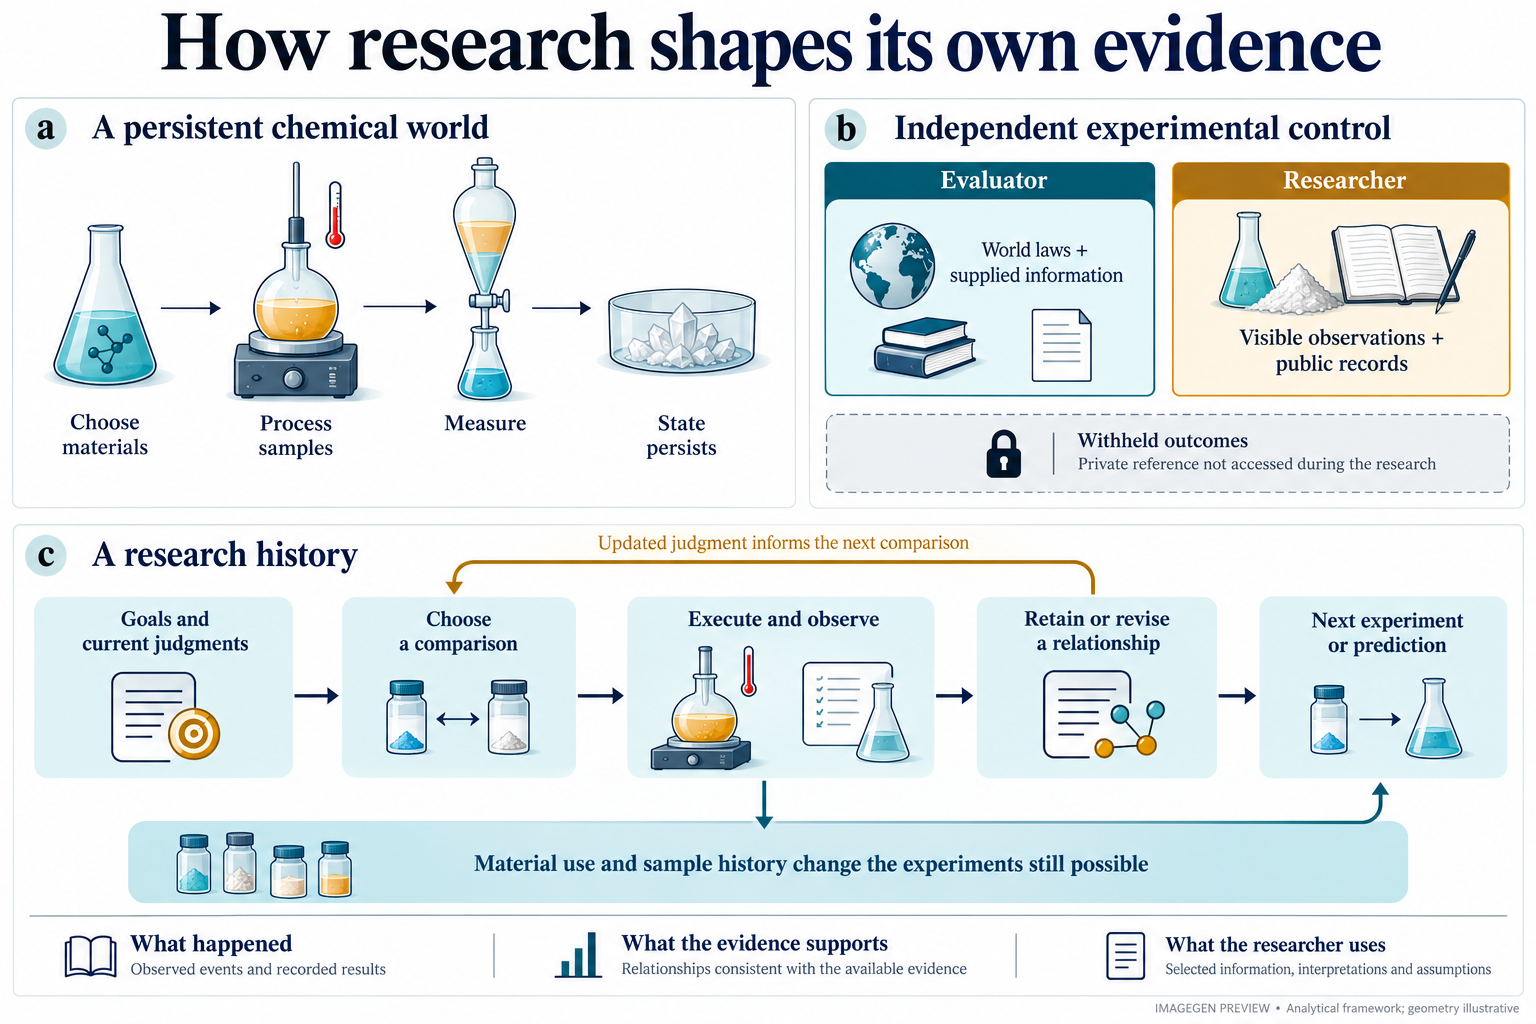
\includegraphics[width=\linewidth,height=.68\textheight,keepaspectratio]{../figures/imagegen-inquiry-focus-20261017/fig01_inquiry.png}}
\caption{Figure 1 \textbar{} Autonomous research shapes its own evidence. a, Agents choose materials, operations and measurements within a persistent chemical world. b, World laws and supplied information are independently controlled while reference outcomes remain withheld. c, Public expectations, chosen comparisons, observations, revised judgments and subsequent actions are connected through a research history. Resources and sample states constrain which experiments remain possible. The diagram is an analytical framework, not a claim that every session follows one cycle. ImageGen preview; geometry is illustrative.}
\end{figure*}

\subsection{The self-organization and adaptation of scientific inquiry}\label{the-self-organization-and-adaptation-of-scientific-inquiry}

Research goals and information create different starting conditions, but their consequences depend on what researchers choose to investigate. In the repeated electrochemical matrix, optimization rather than discovery increases world-equal mean retested recommendation score from 0.4813 to 0.5852 and product yield from 0.1310 to 0.4225. Prediction errors nevertheless increase for score (0.1539 to 0.1829), yield (0.0665 to 0.0781) and Faradaic efficiency (0.1677 to 0.2218), each in all five worlds (Fig. 2a,b). Developing a more effective procedure does not ensure better judgment of new interventions.

Information has similarly differentiated consequences. Under reaction optimization, Aligned rather than Opaque information improves recommendation score from 0.2735 to 0.4429 and yield from 0.5502 to 0.7116. Risk prediction error falls from 0.2389 to 0.1226, whereas conversion error rises from 0.0355 to 0.1595; all four directions occur in all five worlds (Fig. 2c,d). The comparisons concern complete goal or information conditions. They establish the outcomes to explain without identifying one selected history as their sole cause.

\begin{figure*}[t]
\centering
\pandocbounded{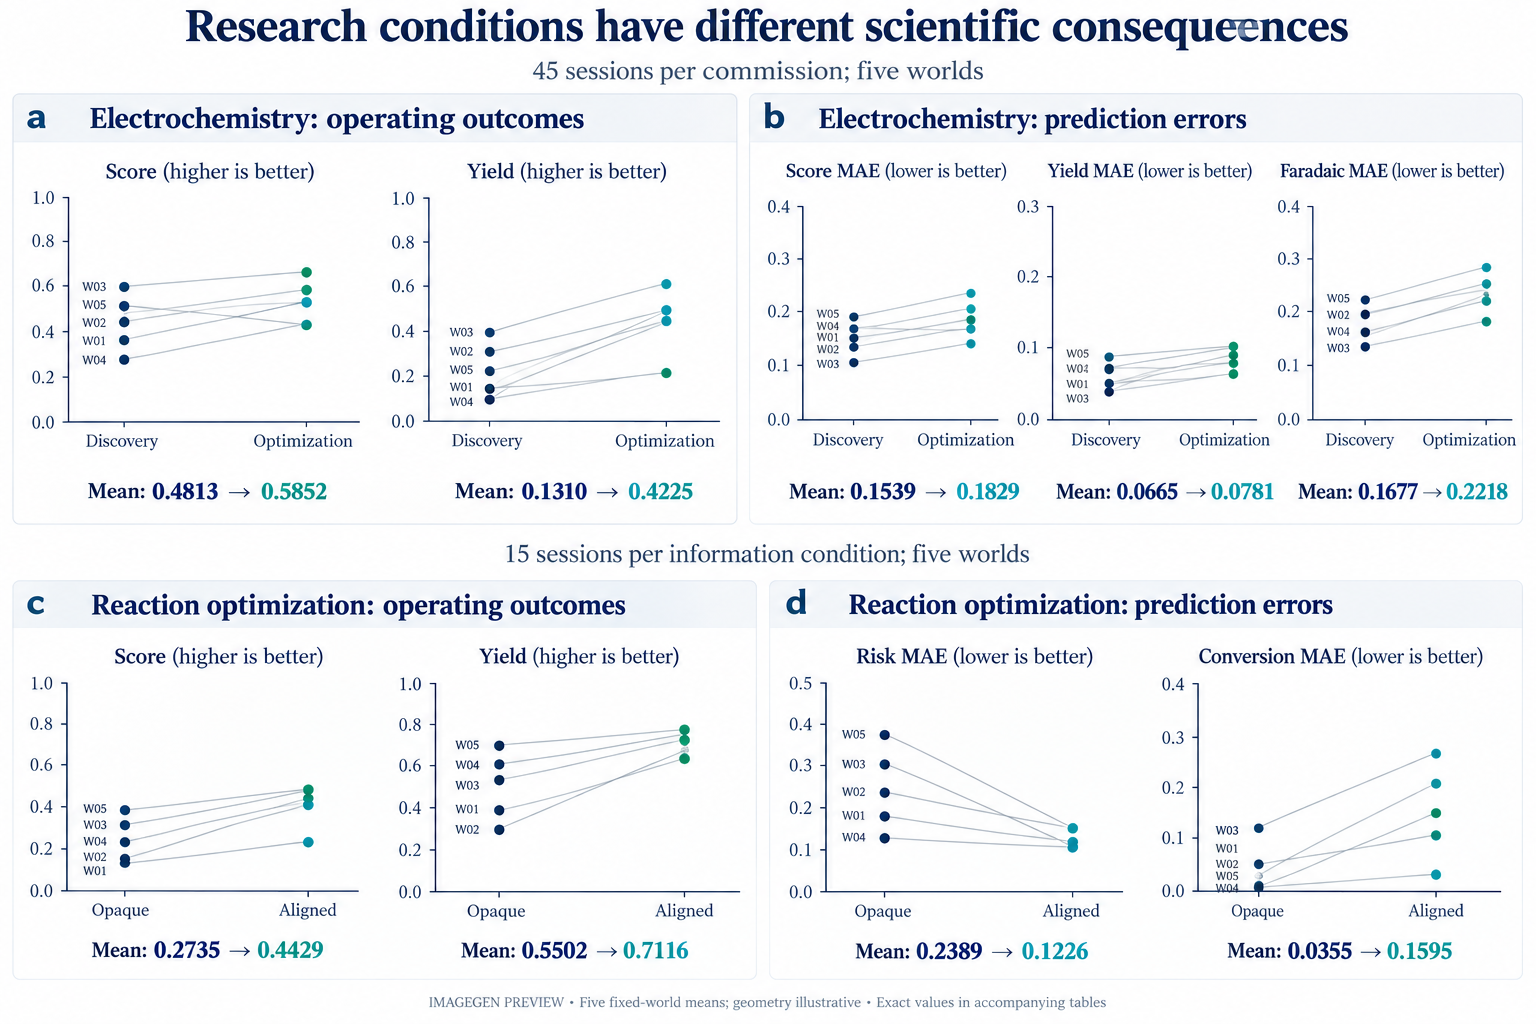
\includegraphics[width=\linewidth,height=.68\textheight,keepaspectratio]{../figures/imagegen-inquiry-focus-20261017/fig02_conditions.png}}
\caption{Figure 2 \textbar{} Goals and information have different consequences for operation and prediction. a,b, Electrochemical discovery-optimization comparisons, forty-five sessions per commission across five fixed worlds and three information conditions. c,d, Reaction optimization under Opaque and Aligned information, fifteen sessions per arm. The preview illustrates within-world comparisons; displayed summary values refer to retained results. Generated dots and lines do not reproduce exact session values, world means or uncertainty. Exact values and available-response denominators are retained in Supplementary Information. ImageGen preview; geometry is illustrative.}
\end{figure*}

Purification study A shows directly how a result changes the organization of inquiry (Fig. 3a). A no-wash procedure gives purity 0.8140 and recovery 0.0479. Increasing the organic-phase amount raises recovery but leaves purity at 0.7886, below the required 0.80. Before batch 11, the researcher predicts that a small 0.005 L wash will cross the purity threshold. It also sets a prospective action criterion: ``if it passes with recovery above 0.0479, replicate it in batch 12.'' This separates an expected scientific response from the condition for pursuing the procedure.

Batch 11 reaches purity 0.8013 but recovery only 0.0441. The first expectation is met, while the continuation criterion is not. Batch 12 therefore repeats the earlier no-wash procedure, yielding purity 0.8149 and recovery 0.0368. The final account recognizes repeatability of qualification alongside variation in recovery, and later predictions retain the observed purity--recovery trade-off. The investigator does not treat improvement in one response as sufficient reason to continue the alternative. Its written criterion, actual test and next choice are connected in time; the near-threshold wash result remains a local observation rather than evidence of robust qualification.

Purification study B exposes a complementary route by which a judgment changes the evidence still obtainable. After four low-recovery batches, the researcher proposes that a feed component was omitted and states that it will add that component in the remaining experiments. The next four batches implement both addition commands, which consume the same shared stock. Stock depletion then prevents the planned temperature experiments. In the final note, the researcher correctly excludes those rejected or blank operations from temperature-response evidence. The interpretation concerns both chemistry and operation semantics, but its practical sequence is clear: a proposed explanation changes material use, and material use changes the remaining research opportunity. The record does not isolate the explanation's effect from every other determinant of that choice.

Two electrochemical histories connect the repeated goal comparison to different uses of local evidence. Electrochemical study A begins with a matched sign comparison: negative potential produces a response where the tested positive setting is effectively inactive. Subsequent batches refine materials and duration on the negative side. The terminal note explicitly limits the sign result to the tested recipe. Yet later numerical forecasts assign near-background responses to untested positive potentials within the examined magnitude range, with intervals missing the references. A stated boundary and its application in new judgments can therefore diverge.

Electrochemical study B, also commissioned to optimize, makes the scope of polarity dependence an experimental question (Fig. 3c). After ten batches of material and duration investigation, the researcher records that the claim of positive-polarity specificity has not undergone a matched reverse-sign test. It reserves a matched reverse-sign test and an exact repeat, writing: ``If negative potential retains high yield, the assumed polarity specificity is rejected''. Batch 11 at −1.0 V retains yield 0.384; the positive recipe and its final repeat give approximately 0.911 and 0.905. The terminal account changes from apparent polarity specificity to polarity advantage, and subsequent forecasts retain reverse-polarity production. This is an explanatory test within optimization, followed by a narrower relationship that remains useful. The two histories belong to different worlds and information conditions, so they illustrate alternative paths without constituting a randomized comparison of testing strategies.

\begin{figure*}[t]
\centering
\pandocbounded{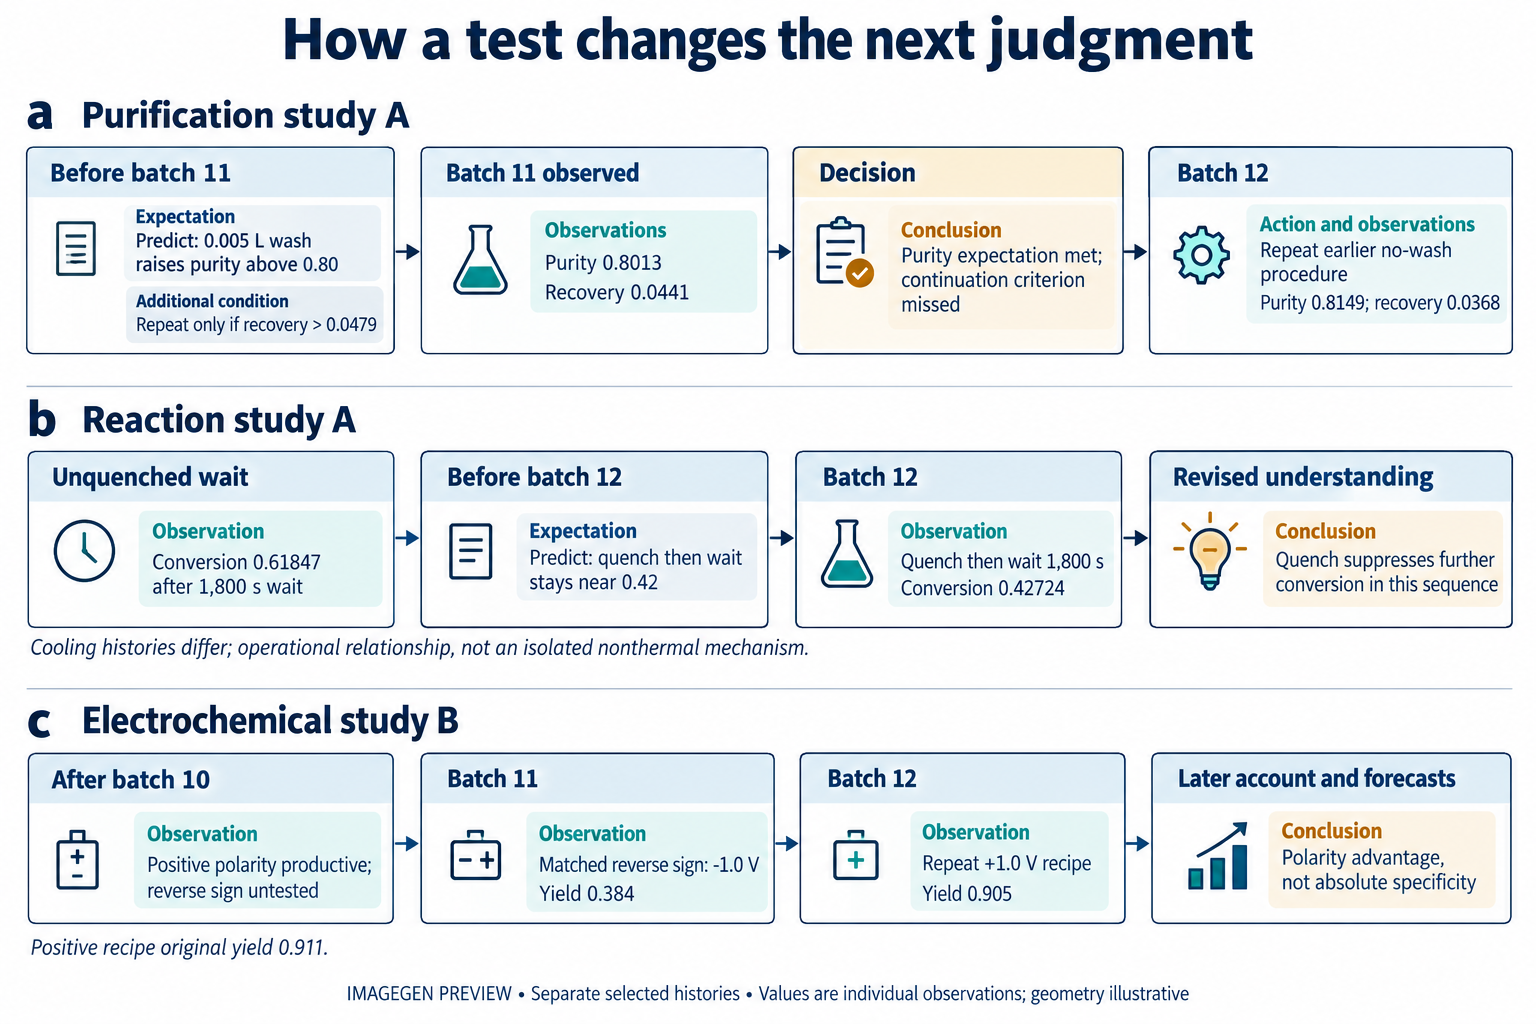
\includegraphics[width=\linewidth,height=.68\textheight,keepaspectratio]{../figures/imagegen-inquiry-focus-20261017/fig03_histories.png}}
\caption{Figure 3 \textbar{} Expectations, tests and subsequent research in three core histories. a, Purification study A: the small-wash purity expectation is met, but recovery misses the prospective continuation criterion; the researcher repeats the earlier no-wash procedure. b, Reaction study A: an unquenched wait motivates a predicted quench-before-wait comparison, followed by a locally supporting result. c, Electrochemical study B: a reverse-sign test retains appreciable production, changing absolute specificity to a polarity advantage; the final batch repeats the positive recipe. Rows are separate selected trajectories. Labels summarize public notes; values are individual observations, not treatment means. Batch and note locations are indexed in Supplementary Information. ImageGen preview; geometry is illustrative.}
\end{figure*}

The three core trajectories provide complementary evidence: applying an existing continuation criterion to a new observation, prospectively testing a local operational expectation, and revising the content of a scientific relationship. They are not replications of a single complete cycle. The central distinction is whether a judgment changes the comparison undertaken and how its result is used. Historical five-model equilibrium campaigns provide a further contrast: some accurate predictions follow direct exploration of a dilute region, while others follow extrapolation from local observations (Extended Data Fig. 7). Those campaigns extend the range of observed paths, but do not add replications to the current matrices or define fixed model traits.

\subsection{The formation and evolution of scientific understanding through experimentation}\label{the-formation-and-evolution-of-scientific-understanding-through-experimentation}

Reaction study A follows an expectation from observation through a new experiment to later use (Fig. 3b). At 390 K and 1,800 s heating, direct termination gives conversion 0.41718. A later batch with the same heating followed by an unquenched 1,800 s wait reaches 0.61847 despite cooling by about 44 K. The researcher treats this as evidence that stopping external heating has not ended the chemical change. Before the final batch, it predicts that quenching before the same wait should preserve conversion near 0.42, rather than the approximately 0.62 unquenched-wait result.

The final batch implements that order and gives conversion 0.42724. The subsequent note retains a local relationship between the quench operation and suppression of further conversion. The new evidence thus changes which part of the processing history the researcher treats as chemically consequential. Later forecasts use this relationship in new procedures, while transfer to unobserved solvent and loading conditions remains less accurate. What has been established is concrete: a prospectively specified operational comparison supports a useful local expectation.

The comparison supports reaction suppression under the tested operation sequence, without separating temperature change from other possible effects (Methods).

The matched-world matrix asks a related question under independent control of underlying chemistry (Fig. 4). Five pairs of aqueous worlds share public framing and selected parameters but differ in coupling to an additional neutral ion pair. Replaying chosen action sequences in their paired worlds shows that every one of thirty sessions acquires at least one observation differing by three assay standard deviations in two response channels. This quantifies physically available information. Whether the researcher recognizes what that information resolves must be examined in its history.

A post hoc analysis of all thirty sessions tests whether final forecasts preserve the paired-world response differences. For each common query, we compare the difference between three-session forecast means with the difference between the original reference means (Fig. 4a--c). Among nonzero reference contrasts, directions agree in 54/57 for pH, 48/57 for dissociation and 39/39 for precipitation; the remaining 3, 3 and 21 contrasts have zero reference differences and remain in the analysis. Where reference differences reach three assay standard deviations, they agree in 48/48, 10/10 and 27/27, respectively; all smaller differences remain in the analysis. The forecasts thus reflect substantial world differences. This result concerns prediction, not unique mechanism identification or an isolated benefit of research: this block has no no-research arm, and starter observations are close but not identical.

In matched-world study A, the researcher states that a sharp precipitation onset with a buffered dissolved response would support a solubility-limited interpretation, while smooth changes would also admit an empirical partition description. After six assays it proposes denser concentration sampling, a central repeat and increased loading; the next six batches implement those choices. The twelve actual observations provide the evidence behind the adopted relation (Fig. 4d; Supplementary Information). Its final account retains a smooth monotone relationship, and its forecast explicitly uses that relationship because no sharp threshold was resolved. Matched-world study B predicts a response to diluting a concentrated sample from 0.75 to 0.375 M and then performs the dilution. Normalized pH rises from 0.08045 to 0.10803. The researcher supports approximate reversibility, while the nearest separately prepared comparator is 0.4 M and the precipitation readings come from different instruments. These records connect specified alternatives to actual comparisons and bounded conclusions; physical distinguishability alone would not establish that connection.

\begin{figure*}[t]
\centering
\pandocbounded{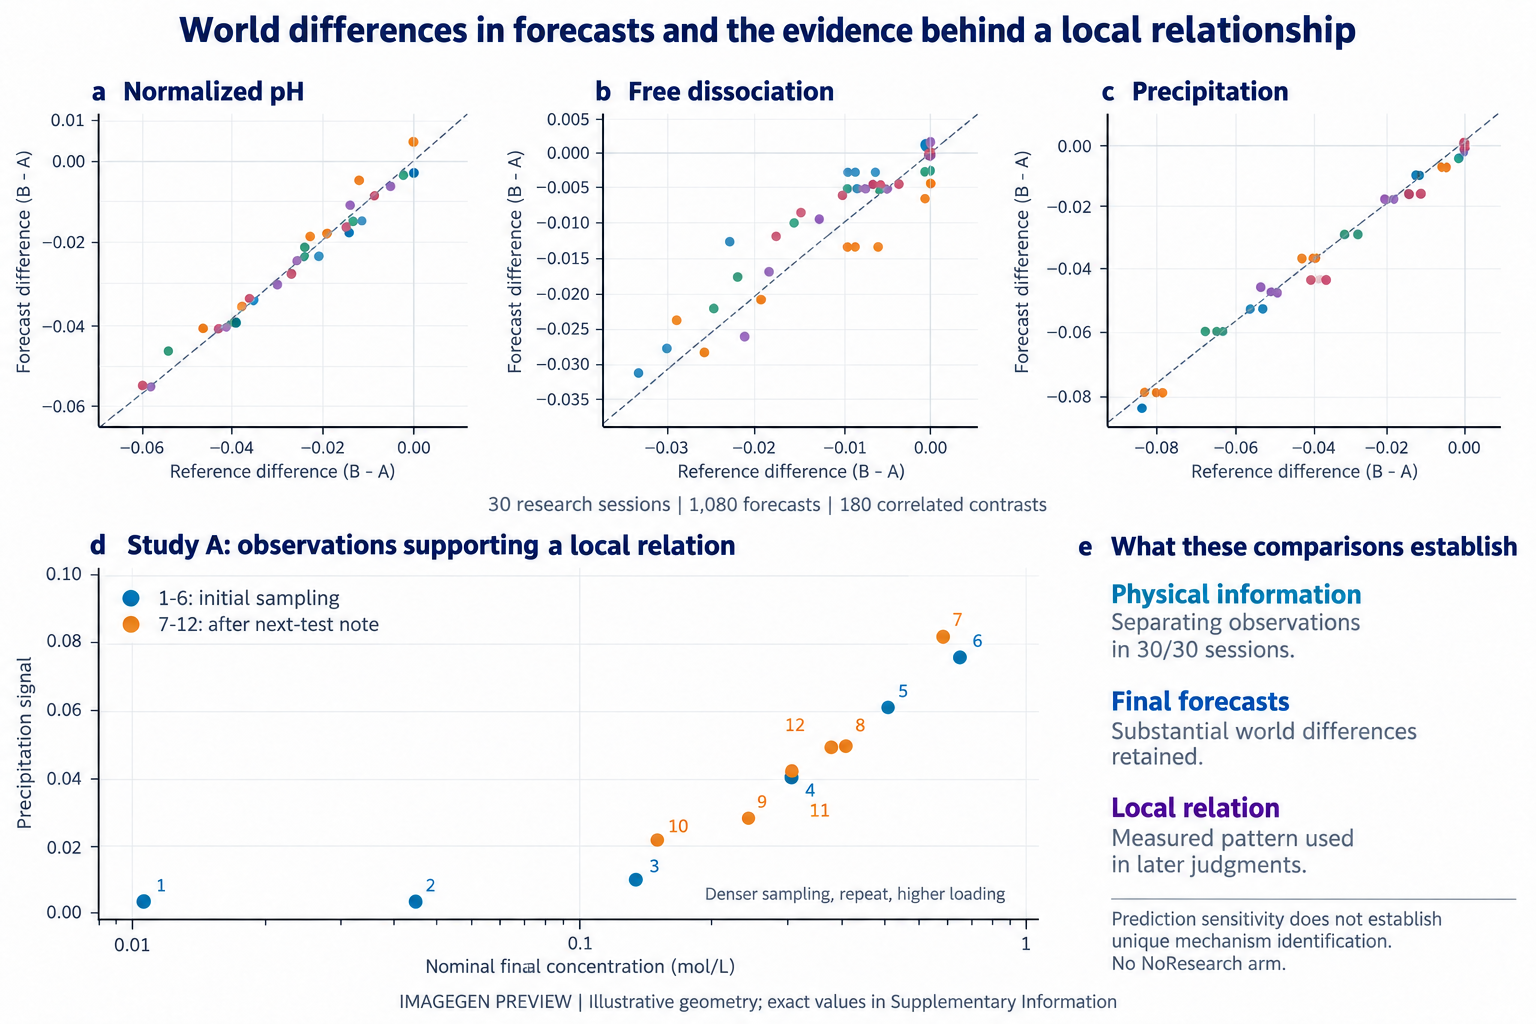
\includegraphics[width=\linewidth,height=.68\textheight,keepaspectratio]{../figures/imagegen-inquiry-focus-20261017/fig04_matched-v2.png}}
\caption{Figure 4 \textbar{} World differences retained in forecasts and observations supporting a local relationship. a-c, Layout preview comparing reference differences between networks B and A with differences between their three-session forecast means. The full analysis retains all 180 correlated contrasts, including zero and small differences; reference values use the original five-observation means. The dashed diagonal denotes equality, not a fitted trend. d, Preview of the twelve-assay history from matched-world study A; batches 7-12 follow its next-test note. Exact conditions and observations accompany the source records. e, Physical information, final prediction sensitivity and local relation formation remain distinct evidence. This block has no NoResearch arm. ImageGen preview; generated coordinates are illustrative, not exact observations or a mechanism-identification rate.}
\end{figure*}

Complementary histories show that learning can also proceed through failed expectations (Extended Data Fig. 8). Stronger mixing defeats a provisional partitioning plateau; a fourth crystallization thermal cycle fails to extend the improvement from the third; further dilution removes recoverable particles and narrows an apparent operating window. These tests contribute through the judgments they revise, even when they do not improve the final procedure. The effects of simultaneously changed factors remain unresolved where the experiments did not separate them.

We follow such judgments within their complete research trajectories. A defensible revision can coexist with an unsupported premise elsewhere in the same session. Supporting cases concern how researchers reconstruct what was performed: some treat rolled-back operations as completed tests, while others explicitly exclude them (Extended Data Fig. 6). In the focal heating case, the public return itself combines success labels with an explicit rollback message and zero time and temperature changes. Its later interpretation therefore concerns interface presentation and remembered experimental history together, rather than an isolated chemical-inference failure. Methods and Supplementary Information preserve the conflicting public signals and distinguish terminal accounts from premises recorded before subsequent action.

Across these histories, understanding develops through observable changes in what is compared, what relationship is supported and what is carried into another decision. These are connected transitions within research. Neither an accurate final answer nor the presence of scientific language establishes that all of them occurred.

\subsection{The nature and conditions of scientific progress in autonomous inquiry}\label{the-nature-and-conditions-of-scientific-progress-in-autonomous-inquiry}

The opportunity matrix measures the consequences of access to research. In each of two systems, five fixed worlds and three fresh sessions per arm compare twelve-batch research with no source experimentation under common Opaque information and assessment. The contrast estimates the complete opportunity to choose experiments, receive feedback and record judgments. It complements the process histories without attributing the difference to a single reasoning activity.

The new crystallization comparison establishes substantial benefits (Fig. 5a). All thirty sessions provide valid forecasts. Relative to no research, world-equal mean absolute error falls from 0.13853 to 0.01661 for purity and from 0.23619 to 0.07641 for size index. Recovery error falls from 0.13532 to 0.11579 and fines error from 0.37683 to 0.30110. For purity, nominal 80\% interval coverage rises from 0.46667 to 0.98333 while width contracts from 0.44744 to 0.09743. The narrower intervals cover more reference outcomes, although coverage above the nominal level is not by itself evidence of calibrated uncertainty. Research experience in these virtual worlds substantially improves subsequent judgments.

\begin{figure*}[t]
\centering
\pandocbounded{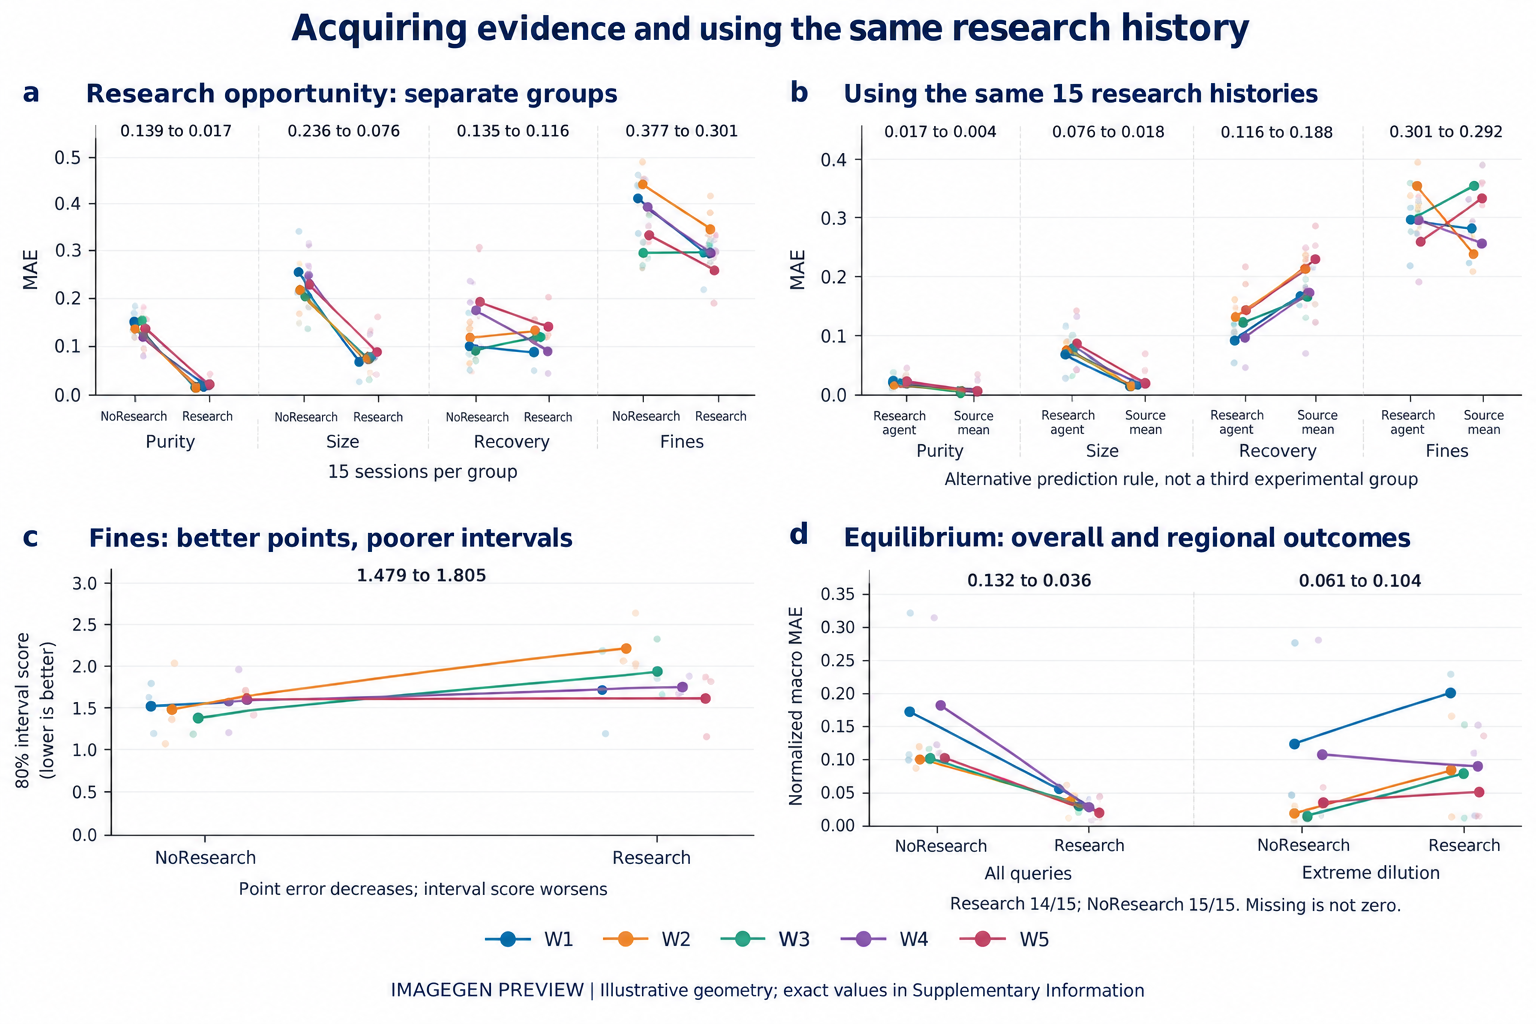
\includegraphics[width=\linewidth,height=.68\textheight,keepaspectratio]{../figures/imagegen-inquiry-focus-20261017/fig05_opportunity-v2.png}}
\caption{Figure 5 \textbar{} Acquiring evidence, using observations and expressing uncertainty. a, Crystallization Research and NoResearch point errors, fifteen valid forecasts per arm. b, Research forecasts compared with a constant reference calculated from the same fifteen source histories and scored on the same targets; this is an alternative prediction rule, not a third experimental arm. c, Fines scores for nominal 80\% prediction intervals (lower is better). d, The separate retained equilibrium comparison, overall and in the prespecified extreme-dilution region: fourteen Research and fifteen NoResearch forecasts. World three has two available Research repetitions; missing outcomes are not zero. Summary labels follow retained results. ImageGen preview; generated session dots and world-connection lines are illustrative, not exact numerical marks, within-agent learning or confidence intervals. Exact values remain in Supplementary Information.}
\end{figure*}

The same cohort distinguishes better point prediction from better uncertainty estimates (Fig. 5c). For fines, coverage falls from 0.42778 to 0.35556 as interval width contracts from 0.68500 to 0.38450. The interval score, which penalizes width and missed outcomes, worsens from 1.4794 to 1.8047 in the world-equal mean, with worsening in every world. Research reduces average fines prediction error, but the resulting intervals express more certainty than their performance warrants. The benefit and the limitation concern the same response in the same comparison.

A second comparison asks what predictions can be obtained from these same research histories (Fig. 5b). For the fifteen Research sessions, the retained source-only mean reference has purity error 0.00450 and size error 0.01786, below the agent's 0.01661 and 0.07641 in all fifteen sessions. The pattern reverses for recovery: the agent's 0.11579 improves on the reference's 0.18828, with an advantage in fourteen sessions. The reference uses only the session's public source observations and is scored on the same targets; it receives no target outcomes for fitting. This is an alternative prediction rule applied to the Research histories, not a third experimental arm or a further stage of learning. A constant reference can suit stable responses without understanding their chemistry; the agent's recovery advantage likewise does not establish a correct mechanism. Together, the two comparisons show that research can be valuable while the predictive value extracted from its observations varies across responses. They do not causally decompose the research effect. The earlier corrected-crystallization diagnostic remains a separate supporting result (Extended Data Fig. 3).

The retained equilibrium opportunity comparison reveals a regional boundary (Fig. 5d). Among fourteen valid Research forecasts and fifteen NoResearch forecasts, overall normalized macro error falls from 0.132086 to 0.035632, with improvement in all five worlds. Error on the three prospectively specified extreme-dilution queries instead rises from 0.061467 to 0.103677, worsening in four worlds; the remaining nine improve from 0.155625 to 0.012950. Allowing the missing Research forecast any error in its legal range does not reverse either aggregate direction (Methods). Local evidence can improve most predictions while leaving its application in another region less reliable. The retained plateau history illustrates one such application without establishing the sole cause of the aggregate reversal (Extended Data Fig. 5).

Information comparisons further specify the conditions of progress. Partitioning phase-fraction errors are 0.04654, 0.05621 and 0.07700 under Aligned, Opaque and MisIndexed information; Aligned improves on MisIndexed in all five worlds. Purification purity errors remain similar across conditions, approximately 0.152--0.154, while MisIndexed has the lowest recovery error. Together with the reaction contrast, these results show that an information package can aid one judgment without improving every response. Historical prior and budget comparisons provide further boundaries in separate cohorts (Extended Data Fig. 1; Supplementary Information).

The quantitative and process evidence answer complementary questions. Opportunity comparisons establish what changes when research is available; the histories show how expectations become tests, results enter choices and useful relationships acquire a scope. Goal and information contrasts show that these consequences depend on how inquiry begins. Scientific progress in these systems includes effective procedures, reliable local relationships, successful transfer and appropriate uncertainty, whose development can diverge within the same investigation.

\FloatBarrier
\subsection{Discussion}\label{discussion}

Autonomous research shapes understanding partly by shaping the evidence from which it develops. The purification trajectories make this relationship concrete. One researcher distinguishes a successful purity prediction from the criterion for continuing a procedure and changes its next experiment accordingly. Another acts on an explanation in a way that depletes stock and removes later opportunities to test temperature. These are different consequences of judgments entering research organization. Evidence acquisition depends on the evolving inquiry, including its objectives, interpretations, resources and operation semantics.

The reaction and electrochemical tests show how this organization can produce scientific progress. A discrepancy motivates a prospective comparison; the result supports an operational relationship or changes an apparently categorical one into a qualified advantage. The empirical contribution lies in tracing what these activities establish and how it is subsequently used. Local relationships can guide further work while some explanatory alternatives and applications remain open.

The crystallization comparisons separate the benefits of acquiring evidence from how effectively it is used. Research produces large gains in purity and size prediction, while a source-only mean gives still lower errors in those same histories. For recovery, the researcher instead outperforms that reference in fourteen of fifteen sessions. The value of a particular use of evidence therefore depends on the response being predicted. Improved fines point predictions coexist with deteriorating interval scores. These findings distinguish the value of acquiring evidence from the quality of its application, and both from uncertainty about unresolved conditions\textsuperscript{12,22,23}. Scientific understanding cannot be inferred solely from whether the final procedure succeeds or the average prediction improves.

This account also clarifies what the designs can explain. Comparisons estimate complete goal, information or research-opportunity conditions; selected trajectories do not identify unique mediators of those effects. Matched-world replay quantifies information under fixed actions, not how another feedback sequence would redirect an agent. A separate fixed-recipe quench comparison measures physical consequences without researcher adaptation (Extended Data Fig. 4). Establishing these distinct contributions allows the paper to explain substantive developments in understanding without requiring one causal mechanism for every case.

The evidence remains limited to programmable worlds and, for the repeated matrices, one model configuration. Fresh sessions do not constitute controlled model-seed replications or independent samples of chemical laws. Public notes locate expressed judgments rather than private cognition, and missing intermediate statements limit temporal inference. All new public histories were read; the seven named histories additionally receive an internal check of quotations, temporal order, implemented comparisons and subsequent use. Selection and interpretation remain retrospective, unblinded and without independent human second-rater validation. The source packet supports such a review but does not substitute for it. Interface ambiguities are retained as part of the research environment rather than attributed solely to scientific reasoning. These boundaries define what can be concluded from the present comparisons and records.

ChemWorld provides an experimental basis for studying how autonomous inquiry develops its own evidential foundation. Researchers do not merely accumulate observations: they change what to compare, which relationships they regard as supported and how they continue. Understanding this development connects the promise of experimental autonomy to a scientific question that can be investigated directly---how exploration produces reliable knowledge, and how that knowledge enables further exploration.

\subsection{Funding}\label{funding}

This work was supported by the Shenzhen Science and Technology Program (AI2026004), the Tsinghua University Initiative Scientific Research Program and the Scientific Research Innovation Capability Support Project for Young Faculty (ZYGXQNJSKYCXNLZCXM-E7).

\clearpage
\onecolumn

\section{References}\label{references}

\protect\phantomsection\label{refs}
\begin{CSLReferences}{0}{1}
\hypertarget{ref-einstein1905electrodynamics}{}
\CSLLeftMargin{1. }%
\CSLRightInline{A. Einstein. Zur elektrodynamik bewegter k{ö}rper. \emph{Annalen der Physik} \textbf{322} 891--921 (1905). https://doi.org/\href{https://doi.org/10.1002/andp.19053221004}{10.1002/andp.19053221004}.}

\hypertarget{ref-douven2025peirce}{}
\CSLLeftMargin{2. }%
\CSLRightInline{I. Douven. Peirce on abduction. \emph{The stanford encyclopedia of philosophy: abduction} (2025). \url{https://plato.stanford.edu/entries/abduction/peirce.html}.}

\hypertarget{ref-tom2024selfdriving}{}
\CSLLeftMargin{3. }%
\CSLRightInline{G. Tom et al. {Self-Driving Laboratories for Chemistry and Materials Science}. \emph{Chemical Reviews} \textbf{124} 9633--9732 (2024). https://doi.org/\href{https://doi.org/10.1021/acs.chemrev.4c00055}{10.1021/acs.chemrev.4c00055}.}

\hypertarget{ref-boiko2023autonomous}{}
\CSLLeftMargin{4. }%
\CSLRightInline{D. A. Boiko, R. MacKnight, B. Kline, and G. Gomes. Autonomous chemical research with large language models. \emph{Nature} \textbf{624} 570--578 (2023). https://doi.org/\href{https://doi.org/10.1038/s41586-023-06792-0}{10.1038/s41586-023-06792-0}.}

\hypertarget{ref-king2009automation}{}
\CSLLeftMargin{5. }%
\CSLRightInline{R. D. King et al. {The Automation of Science}. \emph{Science} \textbf{324} 85--89 (2009). https://doi.org/\href{https://doi.org/10.1126/science.1165620}{10.1126/science.1165620}.}

\hypertarget{ref-burger2020mobile}{}
\CSLLeftMargin{6. }%
\CSLRightInline{B. Burger et al. {A mobile robotic chemist}. \emph{Nature} \textbf{583} 237--241 (2020). https://doi.org/\href{https://doi.org/10.1038/s41586-020-2442-2}{10.1038/s41586-020-2442-2}.}

\hypertarget{ref-macleod2020selfdriving}{}
\CSLLeftMargin{7. }%
\CSLRightInline{B. P. MacLeod et al. {Self-driving laboratory for accelerated discovery of thin-film materials}. \emph{Science Advances} \textbf{6} eaaz8867 (2020). https://doi.org/\href{https://doi.org/10.1126/sciadv.aaz8867}{10.1126/sciadv.aaz8867}.}

\hypertarget{ref-szymanski2023alab}{}
\CSLLeftMargin{8. }%
\CSLRightInline{{N. J. Szymanski et al.} An autonomous laboratory for the accelerated synthesis of inorganic materials. \emph{Nature} \textbf{624} 86--91 (2023). https://doi.org/\href{https://doi.org/10.1038/s41586-023-06734-w}{10.1038/s41586-023-06734-w}.}

\hypertarget{ref-bran2024augmenting}{}
\CSLLeftMargin{9. }%
\CSLRightInline{A. M. Bran et al. Augmenting large language models with chemistry tools. \emph{Nature Machine Intelligence} \textbf{6} 525--535 (2024). https://doi.org/\href{https://doi.org/10.1038/s42256-024-00832-8}{10.1038/s42256-024-00832-8}.}

\hypertarget{ref-dai2024mobile}{}
\CSLLeftMargin{10. }%
\CSLRightInline{T. Dai et al. {Autonomous mobile robots for exploratory synthetic chemistry}. \emph{Nature} \textbf{635} 890--897 (2024). https://doi.org/\href{https://doi.org/10.1038/s41586-024-08173-7}{10.1038/s41586-024-08173-7}.}

\hypertarget{ref-elmachtoub2022spo}{}
\CSLLeftMargin{11. }%
\CSLRightInline{A. N. Elmachtoub and P. Grigas. Smart {Predict, then Optimize}. \emph{Management Science} \textbf{68} 9--26 (2022). https://doi.org/\href{https://doi.org/10.1287/mnsc.2020.3922}{10.1287/mnsc.2020.3922}.}

\hypertarget{ref-shmueli2010explain}{}
\CSLLeftMargin{12. }%
\CSLRightInline{G. Shmueli. {To Explain or to Predict?} \emph{Statistical Science} \textbf{25} 289--310 (2010). https://doi.org/\href{https://doi.org/10.1214/10-sts330}{10.1214/10-sts330}.}

\hypertarget{ref-platt1964inference}{}
\CSLLeftMargin{13. }%
\CSLRightInline{J. R. Platt. {Strong Inference}. \emph{Science} \textbf{146} 347--353 (1964). https://doi.org/\href{https://doi.org/10.1126/science.146.3642.347}{10.1126/science.146.3642.347}.}

\hypertarget{ref-lindley1956information}{}
\CSLLeftMargin{14. }%
\CSLRightInline{D. V. Lindley. {On a Measure of the Information Provided by an Experiment}. \emph{The Annals of Mathematical Statistics} \textbf{27} 986--1005 (1956). https://doi.org/\href{https://doi.org/10.1214/aoms/1177728069}{10.1214/aoms/1177728069}.}

\hypertarget{ref-chaloner1995design}{}
\CSLLeftMargin{15. }%
\CSLRightInline{K. Chaloner and I. Verdinelli. {Bayesian Experimental Design: A Review}. \emph{Statistical Science} \textbf{10} 273--304 (1995). https://doi.org/\href{https://doi.org/10.1214/ss/1177009939}{10.1214/ss/1177009939}.}

\hypertarget{ref-mirza2025chembench}{}
\CSLLeftMargin{16. }%
\CSLRightInline{A. Mirza et al. {A framework for evaluating the chemical knowledge and reasoning abilities of large language models against the expertise of chemists}. \emph{Nature Chemistry} \textbf{17} 1027--1034 (2025). https://doi.org/\href{https://doi.org/10.1038/s41557-025-01815-x}{10.1038/s41557-025-01815-x}.}

\hypertarget{ref-majumder2025discoverybench}{}
\CSLLeftMargin{17. }%
\CSLRightInline{B. P. Majumder et al. {DiscoveryBench: Towards Data-Driven Discovery with Large Language Models}. \emph{{International Conference on Learning Representations}} \textbf{2025} 4556--4579 (2025). \url{https://proceedings.iclr.cc/paper_files/paper/2025/file/0d70af566e69f1dfb687791ecf955e28-Paper-Conference.pdf}.}

\hypertarget{ref-wang2022scienceworld}{}
\CSLLeftMargin{18. }%
\CSLRightInline{R. Wang, P. Jansen, M.-A. Côté, and P. Ammanabrolu. {ScienceWorld: Is your Agent Smarter than a 5th Grader?} \emph{Proceedings of the 2022 conference on empirical methods in natural language processing} 11279--11298 (2022). https://doi.org/\href{https://doi.org/10.18653/v1/2022.emnlp-main.775}{10.18653/v1/2022.emnlp-main.775}.}

\hypertarget{ref-jansen2024discoveryworld}{}
\CSLLeftMargin{19. }%
\CSLRightInline{P. Jansen et al. {DiscoveryWorld}: A virtual environment for developing and evaluating automated scientific discovery agents. \emph{Advances in neural information processing systems} \textbf{37} (2024). https://doi.org/\href{https://doi.org/10.52202/079017-0324}{10.52202/079017-0324}.}

\hypertarget{ref-gandhi2025boxinggym}{}
\CSLLeftMargin{20. }%
\CSLRightInline{K. Gandhi et al. {BoxingGym}: Benchmarking progress in automated experimental design and model discovery. (2025). \url{https://arxiv.org/abs/2501.01540}.}

\hypertarget{ref-chen2025physgym}{}
\CSLLeftMargin{21. }%
\CSLRightInline{Y. Chen, P. Piękos, M. Ostaszewski, F. Laakom, and J. Schmidhuber. {PhysGym: Benchmarking LLMs in Interactive Physics Discovery with Controlled Priors}. \emph{{Advances in Neural Information Processing Systems}} \textbf{38} (2025). https://doi.org/\href{https://doi.org/10.52202/085713-1556}{10.52202/085713-1556}.}

\hypertarget{ref-gneiting2007scoring}{}
\CSLLeftMargin{22. }%
\CSLRightInline{T. Gneiting and A. E. Raftery. {Strictly Proper Scoring Rules, Prediction, and Estimation}. \emph{Journal of the American Statistical Association} \textbf{102} 359--378 (2007). https://doi.org/\href{https://doi.org/10.1198/016214506000001437}{10.1198/016214506000001437}.}

\hypertarget{ref-ovadia2019uncertainty}{}
\CSLLeftMargin{23. }%
\CSLRightInline{Y. Ovadia et al. {Can you trust your model's uncertainty? Evaluating predictive uncertainty under dataset shift}. \emph{{Advances in Neural Information Processing Systems}} \textbf{32} (2019). \url{https://proceedings.neurips.cc/paper_files/paper/2019/file/8558cb408c1d76621371888657d2eb1d-Paper.pdf}.}

\end{CSLReferences}

\clearpage

\section{Methods}\label{methods}

\subsection{Worlds, interfaces and experimental units}\label{worlds-interfaces-and-experimental-units}

ChemWorld compiles compatible process components into persistent virtual chemical environments. The public contract specifies materials, legal operations, instruments, resources and task objectives. Private parameters determine each world's responses. Agents access the laboratory and public records, without evaluator state, simulator code, private parameters or withheld reference outcomes. Operations change samples; measurements may consume material. Candidate transitions are validated before commitment. Rejected operations do not constitute the requested physical intervention, although attempts can consume contract-defined allowances. Exact replay checks environment transitions, not regeneration of model decisions.

The broad study covers electrochemistry, partitioning, reaction and thermal processing, aqueous equilibrium, reaction-coupled crystallization and purification. These are controlled virtual systems, not experimentally validated predictions for named physical substances. The integrated repeated design covers all six systems through complementary matrices. Five fixed worlds recur across arms and repetitions; their parameters, initial states and keyed observation mappings are fixed. Repetitions are fresh model sessions, not independent world draws or controlled model-seed replications. The model interface does not expose a usable sampling seed. Repeated identical interventions can share keyed observations, so they are not independent noise samples.

\subsection{Integrated matrices and new-session coverage}\label{integrated-matrices-and-new-session-coverage}

The integrated coverage design contains 450 planned researcher sessions in four matrices, combining a new 300-session block with 150 retained sessions. The objective--information matrix uses electrochemistry and reaction processing, each with five worlds × three information conditions × two commissions × three sessions, or ninety per system. The process matrix uses partitioning under discovery and purification under optimization, each five worlds × three information conditions × three sessions, plus the retained forty-five equilibrium and forty-five corrected-crystallization sessions. The opportunity matrix comprises thirty new crystallization sessions and thirty retained equilibrium sessions: five worlds × Research/NoResearch × three sessions, all Opaque. Thirty retained matched-world sessions form the fourth matrix. The retained 150 and the historical broad 300 are distinct from the new 300; a shared coverage structure does not make their protocols or periods identical.

New participants use gpt-5.6-sol at medium requested reasoning effort. Source studies allow twelve batches; the fifteen no-research participants receive none. Scientific accounts, twelve-query predictions and retrospectives are sealed in order without reference-truth feedback. The 300 planned sessions yield 288 complete chains, 298 valid forecast stages, 3,379/3,420 source final assays and 898/900 valid sealed stages. Electrochemistry completes 90/90 chains and 1,080 assays; reaction processing completes 88/90 chains and 1,080 assays, with 88 valid forecasts; partitioning completes 45/45 chains and 540 assays; purification completes 35/45 chains and 499/540 assays but retains all forty-five forecasts; crystallization completes 30/30 chains, including all thirty forecasts and 180 research assays. The new source and recommendation records have 285 and 240 verified replay receipts, respectively.

Ten purification sessions retain material-exhaustion shortfalls rather than replacement histories. One reaction forecast is absent after tool-budget exhaustion and another is invalid because its intervals violate the assessment requirements. All corresponding operations and later available accounts are retained. Four explicit service interruptions are retried after the primary queue, under the user's predetermined technical-retry rule; every interrupted attempt remains in the ledger and does not add a scientific unit. Earlier runtime-development attempts are separate from this block. No completed scientific outcome is replaced because of its score. The manuscript compilation performs no model or simulator experiment.

\subsection{New-matrix measurements and aggregation}\label{new-matrix-measurements-and-aggregation}

Each response retains its native assessment definition. Electrochemistry and purification use a single keyed final observation as reference; partitioning uses noiseless presampling phase fractions; reaction processing uses a five-observation mean for point error and all sixty reference observations across twelve queries for coverage; crystallization uses noiseless preassay responses and initial-charge recovery. Partitioning intervals are nominal 90\%, whereas the other systems use 80\%. The two partition fractions are complementary, not independent evidence. No cross-response or cross-system scientific-ability score is formed.

Response errors and interval diagnostics are computed per session. Within a condition, available sessions are averaged within each fixed world and the five worlds receive equal weight. The electrochemical commission comparison further averages the three information conditions within each world; all forty-five forecasts per commission are available. The reaction Opaque--Aligned optimization comparison uses fifteen valid forecasts per condition. Other reaction cells with missing forecasts retain fourteen of fifteen and are explicitly marked. Purification uses available forecasts even when the source budget is incomplete. Full-grid estimates remain unavailable when planned responses are missing; available-case values do not impute zero error. Repeated sessions, queries and responses share worlds and are not treated as independent draws for confidence intervals or significance tests. Three repetitions per fixed cell describe variability, not a population reliability rate.

Operating comparisons use independent retests of sealed recommendations. They are distinct from predictions under new query interventions. Scores and yields retain their public definitions and are averaged separately. Interval width, empirical coverage and, where present in the retained evaluator, the proper interval score are reported alongside point error. For the new crystallization opportunity comparison, the score uses alpha = 0.2 and its legal response scale. Research and NoResearch have the same scientific framing and sealed assessment, with research additionally supplying an experimental budget, experience and recording opportunity. Their difference estimates this complete package, not a specific reasoning operation.

\subsection{Full reading of the new research histories}\label{full-reading-of-the-new-research-histories}

All 300 new sessions are read, including the fifteen no-research accounts, all 873 notebook versions and 31,922 public operations. The evidence contains 899 nonempty sealed payloads: one includes an invalid forecast, so there are only 898 valid stages; one forecast payload is absent. Coverage comprises electrochemistry (268 notes; 7,647 operations), reaction processing (293; 7,917), partitioning and purification (262; 13,253), and crystallization (50; 3,105). The retained per-session readings verify 1,363 quotations against public records. Missing notes, unsuccessful tests, rejected requests, terminal revisions and later retrospective admissions remain visible. Reading coverage is not an explanation-success denominator.

For each focal judgment, analysis distinguishes the stated phenomenon, candidate explanation or empirical expectation, its first recorded appearance, prospective consequence, actual committed intervention, measurement, revised standing and later use. A conditional plan is not counted as an executed test. Subsequent predictions are not retroactively inserted into earlier notes. A terminal explanation can support a claim about later prediction, but cannot by itself establish an earlier influence on source actions. Source-time public contracts and the frozen execution semantics distinguish rejected requests, rolled-back transitions and task-quality failures. In particular, a reaction-risk threshold does not imply rollback, and direct heating and controller configuration have different public temperature limits. Quench changes temperature and risk and advances the clock without additional reaction integration; waiting before quench may continue chemistry. Reaction study A compares different cooling histories, so its quench-before-wait result supports a local operational relation without separating thermal and nonthermal effects. The selected crystallization seed review compares requested and committed amounts, rather than treating repeated rejected requests as dose.

All histories receive semantic reading, while illustrative claims are selected retrospectively for their explanatory relevance. Multiple claims can coexist within a session with different support and outcomes. We trace individual judgments within complete trajectories, retaining session and world levels for comparisons. The analysis does not infer private cognition or assign one success label to a whole session. Interpretation and source verification are performed within the assistant analysis workflow; there is no independent human coding, blinding or second-rater reliability estimate. The earlier action-linked windows and selected explanation histories below retain their original definitions and denominators.

\subsection{Same-cohort source references and execution-state interpretation}\label{same-cohort-source-references-and-execution-state-interpretation}

We additionally summarize the source-only references already stored with the fifteen new crystallization Research results. This is a post hoc analysis of retained outputs, with no model or simulator execution. The constant reference averages each session's response-complete public final-assay records; the existing nearest-neighbour reference selects the source recipe nearest to the query in the original public recipe-feature space. Targets are used only for scoring. Response completeness requires numeric values for all four assessed responses, irrespective of their values or task success: 179 of 180 source assays meet this rule; one assay in world 1, repetition 3 lacks the full response vector, leaving eleven fitting assays there. All fifteen sessions and 180 queries per response remain in the analysis. We report mean absolute error against the same noiseless preassay targets as the agent, averaging sessions within worlds and then worlds equally. These point-only references assess use of available observations and are distinct from the NoResearch arm. Per-session errors, fitting counts and source means are retained in the portable archive. This is a comparison of prediction rules on identical histories, not a third experimental group, a measure of private understanding or a causal decomposition of the research-opportunity effect.

For the supporting heating-reconstruction case, the visible return contains outer \texttt{ok:\ true} and \texttt{experiment\_completed:\ true}, but also \texttt{transaction\_status:\ rolled\_back}, an explicit rollback error and zero changes in temperature and time. The two requested 600 s operations therefore do not establish 1,200 s of chemical exposure. The conflicting public labels are preserved alongside the later account and forecasts; this case does not isolate agent reasoning from interface ambiguity. Another session explicitly excludes rolled-back heat from chemical interpretation. Controller and direct-heating limits are checked against their distinct public contracts. These execution checks locate evidential differences, rather than treating every discrepancy as a chemical misconception.

\subsection{Historical and retained evidence layers}\label{historical-and-retained-evidence-layers}

The historical broad pool contains 240 Sol-medium campaigns and 60 additional equilibrium campaigns from Luna, Terra, GPT-5.5 and Astra, requested at medium reasoning effort. The five-model equilibrium comparison includes fifteen Sol campaigns already in the 240. Requested model labels do not establish equal realized computation. The original 240 include 60 electrochemical, 30 partitioning, 60 reaction, 45 equilibrium, 30 crystallization and 15 purification campaigns. They retain 3,597/3,600 final assays, all 720 assessment stages and 238 protocol-conforming campaigns under their original rules. The additional sixty retain 720 batches and 240 stages. Two original source-completion failures remain included. Earlier selected notebook studies comprise another 24 sessions and are not pooled into the broad or retained equilibrium--crystallization process cohort.

The retained equilibrium--crystallization process cohort combines the 45 equilibrium sessions from the earlier 48-session block and its 42-session extension with a complete replacement block of 45 crystallization sessions under a consistent recovery description. Each system covers five worlds, Opaque/Aligned/MisIndexed information and three sessions per cell, with twelve research batches per session. Equilibrium retains 39 complete chains and 41 valid forecasts; corrected crystallization retains 41 and 42, respectively. The combined retained denominator is 90 sessions, 80 complete chains and 83 valid forecasts. Old crystallization sessions remain protocol-affected historical evidence. They are not added to the replacement sessions when calculating current outcomes or process frequencies.

Corrected crystallization has 510/540 source batches, 125/135 assessment stages, 145 notebook versions and 42 recommendation retests. All 45 source trajectories and 42 retests pass replay. Four incomplete chains remain: three lack forecasts, and one retains a valid forecast but lacks the subsequent retrospective. The equilibrium subset and the separate opportunity block retain their own failure tables. Missing outcomes are not set to zero, and later favourable outcomes do not replace completed results. Evidence integration does not change the original development or qualification status of any block.

\subsection{Information, autonomy and recording}\label{information-autonomy-and-recording}

Historical goal comparisons pair independent discovery and optimization campaigns within world, information arm, batch budget and prior locus. Electrochemistry contributes thirty pairs across twelve- and twenty-four-batch conditions; reaction processing contributes thirty across parameter- and structural-prior blocks at twelve batches. Operating outcomes are independent retests of sealed recommendations. The joint-outcome counts use public-score prediction MAE, whereas the reaction prior comparison uses the mean across its six normalized response errors. These outcomes are not interchanged. Budget comparisons likewise concern independent sessions with complete resource envelopes; they do not estimate the effect of continuing the same investigation.

The historical five-model equilibrium comparison contains five worlds, three information arms and one twelve-batch campaign per cell: seventy-five campaigns, including the fifteen Sol campaigns already counted in the broad study. The 1 mM threshold descriptively summarizes the lowest positively loaded nominal concentration assayed; it is not a discovery criterion. Concentration is based on nominal recipe loading, and the three dilute assessment queries are shared across configurations. Forecast errors, original prediction intervals and acquired evidence are retained for all arms. The selected Astra and electrochemical trajectories are retrospective process illustrations, with scientific accounts written after experimentation; they are not contemporaneous notebook records or additional replications. Complete historical design, response tables and case values remain in Supplementary Information.

Opaque supplies the public task and operational context without the additional instance dossier. Aligned supplies partial information appropriate to the system. In equilibrium, this includes an effective-acidity interval and an anchored local dilution relationship. MisIndexed uses another world's archival relationship with the same format and qualification. In crystallization, Aligned gives nominal descriptors for anonymous materials; MisIndexed swaps solvent S1/S3 descriptors while preserving S0, S2 and catalyst descriptors. Neither dossier specifies the complete world law.

The original equilibrium Opaque/Aligned sessions precede its MisIndexed extension. Corrected crystallization is a later complete block. These descriptive comparisons are not all concurrently randomized treatments, and new versus old crystallization is not an estimate of the causal effect of correcting the prompt. The retained equilibrium opportunity comparison uses a common contemporaneous protocol, described below.

Agents choose operations, quantities, measurements, repetitions and grouping within fixed budgets. Equilibrium permits twelve source batches, 180 operation attempts, twelve intermediate instruments and twelve final assays; crystallization uses its fixed twelve-batch materials envelope and 720-attempt ceiling. A notebook role asks for an initial testable expectation when available; subsequent updates are agent-selected, without a write-every-batch requirement or automatic reinjection. The role may influence research and is not assumed passive. Notes retain version and public-event cursor. These public records do not expose private cognition. Absence of a notebook-read tool call does not establish absence of access to the conversation's earlier content.

\subsection{Assessments and recovery definition}\label{assessments-and-recovery-definition}

After source research and any operating recommendation, agents seal a scientific account, answer twelve fixed new-intervention queries without laboratory tools and then reflect without truth feedback. Equilibrium includes a structured supplemental assessment. The evidence notation K1/Q/K2/EQS denotes these stages. Queries are hidden during research; post-assessment proposals are not treated as executed source experiments.

Equilibrium errors compare predictions with the mean of five reference observations per query. Coverage checks all five observations. Crystallization uses the noiseless full-process response immediately before final-assay sampling; source observations are noisy. The corrected block retains sixty reference batches, numerically matching the earlier reference outcomes, and separately retests each available committed recommendation.

The corrected recovery definition is seed-excluded recovered solid target divided by the tracked initial reagent charge, in moles, clipped to {[}0,1{]}. Source instructions, prediction prompts, observations and scores now refer to this same full-process quantity. The internal crystallization-stage metric instead divides by target product before separation. Earlier process instructions described this latter denominator while observations and scoring used initial reagent charge. Original scores are preserved as protocol-affected diagnostics; they do not enter the corrected cohort. That corrected block was rerun in full rather than retrospectively relabelling those scores.

Quality requires particles, purity at least 0.80 and fines at most 0.50; joint recommendation success also requires corrected recovery at least 0.10. Corrected joint counts are 13/15 Opaque, 10/14 Aligned and 10/13 MisIndexed among available retests, against fifteen planned sessions in each arm. Particle size is the public index min(d50/250 micrometres, 1); its error is not measured in micrometres.

\subsection{Research paths and process interpretation}\label{research-paths-and-process-interpretation}

We trace publicly stated relationships and expectations, actual experiments, acquired observations, revisions and subsequent uses. A scientific account or an accurate forecast alone cannot establish this sequence. Interpretation is based on specific histories, not a general reasoning-ability scale. Five named core histories come from the new block: Purification studies A and B, Reaction study A and Electrochemical studies A and B. Supplementary Information maps their stable labels to information conditions, complete public records, note revisions, operation positions and batch sequence. Matched-world studies A and B retain their separate block's identities and anchors. Selection follows complete reading and remains retrospective. The earlier 92 action-linked windows describe recording coverage in the retained equilibrium--crystallization cohort; the equilibrium opportunity case is outside that window cohort.

For the retrospective explanation-history panel, selection is fixed to the focal equilibrium opportunity session and the four corrected-crystallization cases already illustrated in the preceding manuscript: lower charge, interpolation, and the two contrasting seed accounts. We trace seven related judgments across these five sessions, retaining all notebook versions, including terminal revisions. Fields distinguish the phenomenon, a candidate or expectation actually stated by the agent, first appearance, conditional prediction, executed operations, observations, subsequent standing and later use. Missing conditional statements are left missing rather than supplied by the analyst. The equilibrium loading expectation, component hypothesis and background interpretation are connected strands of one inquiry, not three independent discoveries. The panel is not sampled to estimate frequencies; no explanation-level prevalence or reliability denominator is inferred from the window counts.

The focal operation-semantics check uses the retained execution version and trajectory's mechanism identity, not current runtime assumptions. That world's single non-catalytic feed is selected both by the reagent operation and by component 0; both add to the same initial-amount ledger read by the equilibrium response calculation. Switching these commands at equal loading therefore does not switch chemical identity. Final nominal concentrations in Extended Data Figure 5 divide committed added moles by total added solvent volume; the staged-dilution batch is plotted at its final 0.8 mol/L. No new simulator calls are required for this inspection. Proposed low-loading and orthogonal measurements remain unexecuted in the retained source history. The scope of the resulting plateau is assessed independently of the agent's proposed mechanism.

Retrospective path extraction covers sixty historical electrochemical, forty-five equilibrium and forty-five corrected crystallization sessions. Fifty within-world condition contrasts retain goal, budget, information and cohort. Counts use committed operations; solvent coverage includes additions during resuspension. Rejected attempts do not establish successful material use. Interrupted sessions remain in the planned denominator.

Structured extraction considers all 178 adjacent pairs among 268 notebook versions in the retained 90 sessions. Eligibility requires an earlier note, at least one new committed final assay before the next note, and a committed research operation after that later note; measurement and termination alone do not satisfy continuation. All 178 pairs contain new assays. Ninety-two have the required continuation: 34 equilibrium and 58 crystallization windows in 30 and 35 sessions, respectively. The other 86 pairs (44 equilibrium, 42 crystallization) have no later committed research action and remain available in the evidence archive. The 25 sessions without a complete window are not classified as having learned nothing.

Eligibility is computed from event timing before semantic plan matching, without testing whether a proposed action succeeds. Nevertheless, the rule conditions the sample on continued committed research and excludes terminal revisions from this particular action-linked denominator. All 92 eligible windows are coded. Labels concern one selected immediate plan, not every proposal in a note: 83 matched, seven partly matched and two without an explicit next plan; corrected crystallization contributes 52 matched and six partly matched. Full notes retain abandoned, rejected and altered proposals even when another selected action matches. All 182 update/plan quotations and their assay/action cursors are verified against source records. The archive includes every adjacent pair, selected code, full note and execution history.

A further internal review covers the five named new histories and two named matched-world histories. It checks exact quoted wording, note cursors relative to executed comparisons, operation arguments, measured outcomes and later accounts or forecasts. The public packet retains the full notes, batch actions and scientific posttests alongside a supported finding and scope boundary for each case. This review uses the same assistant workflow, with prior knowledge of the outcomes; it is not blinded or independent.

The same analyst performs coding and internal scientific review. There is no independent second-rater agreement estimate, blinding or claim of adjudicated mechanism prevalence. The team has assigned review to this workflow; completed internal review is distinguished from independent replication. Counterexamples include warranted retractions, correct recognition of unexecuted tests and accurate but explicitly conjectural extrapolation. Selection of illustrative cases is retrospective.

\subsection{Matched chemical worlds and explanatory histories}\label{matched-chemical-worlds-and-explanatory-histories}

The additional prospective block contains five parameter pairs, two chemical networks and three fresh Sol-medium sessions per world: thirty planned sessions. Network A couples weak-acid dissociation to direct free-ion precipitation; B adds neutral aqueous ion pairing. Within each pair, acid dissociation, solubility-product, cation, activity and initial-state parameters are matched, along with the public operational contract. Two actual starter assays, each using 6 × 10⁻⁷ mol in 0.080 or 0.075 L, are supplied before autonomous research. The paired noise-free responses differ by no more than one declared final-assay standard deviation in each channel. Participants receive chemical framing and loading, dilution and scale dimensions, but not the private network identity or parameters. The initial notebook therefore follows supplied observations, not an evidence-free pretest.

Qualification of the implemented candidate covers 230 physical states and assays, thirty exact replays and 120 runtime mean checks. Five bounded nuisance refits do not adequately fit network B with the tested direct-network family; this check does not prove identifiability against all alternative explanations. An earlier failed physical candidate remains separate. These checks concern the world's implemented information structure, not agent learning.

Each session has twelve autonomous batches followed by a sealed scientific account, twelve query forecasts and a retrospective without truth feedback. The queries are withheld during research, although agents can visit corresponding physical conditions. All thirty sessions complete all stages: 360 source final assays, ninety sealed stages and 1,080 query-response predictions. Eighty notebook versions comprise twenty sessions with three notes and ten with two. Thus continuous midpoint revision cannot be assumed in every session. Three fresh sessions per world share fixed observation keys; the model sampling seed is unavailable.

Every committed source action sequence is replayed in its own and the paired world: thirty source replays and sixty own/partner trajectories pass. Separation is the absolute difference between noise-free response means divided by the final-assay standard deviation: 0.002 for normalized pH and 0.006 for each fraction. Of 360 final assays, 326 separate at least one channel by three standard deviations and 158 separate at least two; all thirty sessions include an assay of the latter kind. This threshold describes physical information, not statistical significance or the researcher's recognition of a mechanism. Counterfactual replay fixes actions and does not estimate how an agent would adapt to different observations.

Forecast errors use the mean of five retained reference observations per query; intervals are evaluated against all five observations, which are shared across sessions in the same world. Session values are averaged within each world, then the ten worlds equally. Intervals are nominal 80\% prediction intervals, not confidence intervals for means. Their high empirical coverage must be read alongside their widths and does not by itself establish calibration. This block has no no-research arm and uses different chemical laws from the opportunity comparison.

A post hoc forecast-contrast analysis retains all 1,080 predictions. For each of five parameter pairs, twelve common queries and three responses, it subtracts the mean of the three A-world forecasts from the mean of the three B-world forecasts and compares that difference with the corresponding difference between five-observation reference means. All 600 executed reference action sequences are checked against the common query definitions. All 180 contrasts are displayed; tied or opposing directions are not removed. A descriptive subset uses absolute reference gaps of at least three declared single-assay standard deviations (0.002 for pH and 0.006 for fractions), reusing the physical separation scale rather than a significance threshold. This post hoc subset is not a sample-selection rule for the main analysis. Query contrasts share worlds and several target concentrations; three sessions within each world are fresh draws, not model-seed pairs. The analysis measures final forecast sensitivity to world differences, not identification of the true network, a change from baseline cognition, or the isolated effect of research. Supplied starter observations are close but not identical.

All eighty notes and ninety sealed stages are read with their executed actions. Sixty-seven selected focal histories retain 365 verified quotations. A separate retrospective reading covers 105 existing sessions and 309 notes, tracing 112 selected histories and 218 note anchors; four selected sealed follow-ups add thirteen anchors. The 105 are the retained ninety plus fifteen research-opportunity sessions, not additional experiments. Histories can overlap within a session and include terminal revisions. They are descriptive units selected for explanatory relevance, not independent discoveries or population frequencies. Initial expectations, candidate explanations, empirical relations, executed tests and subsequent uses remain distinguishable; absent causal or conditional statements are not supplied by the analyst.

Source operations retain 1,901 attempts: 1,893 committed, six rolled back and two rejected by validation. Another 131 recovered tool failures are counted separately. The first launch attempt contains four startup failures, twenty-six unstarted sessions and no scientific operations; after a thread configuration repair, the entire thirty-session block restarted. All earlier failures and resource records are retained. No completed scientific outcome is replaced because of its value.

\subsection{Source-only forecast references}\label{source-only-forecast-references}

Two transparent references are computed for each valid corrected-crystallization forecast using only that researcher's successful source final assays. The first averages all available assays. The second averages assays whose exact set of committed solvent identifiers matches the query, falling back to the overall mean when none match. Solvent sets include successful solvent additions and resuspension, excluding rejected actions. The fitting function receives no test truth. These references are descriptive calculations, not separately trained agents or mechanistically complete baselines.

There are 42 valid sessions and 504 queries. Same-solvent fallback occurs in 186/504 queries: 1/180 Opaque, 95/168 Aligned and 90/156 MisIndexed. Matching does not control thermal history, quantities or final liquid composition. References have no predictive intervals. Each response is reported in its own public scale; no combined score is formed across recovery, purity, size and fines.

The added distribution analysis uses those same 42 valid sessions and their 504 source final assays. For each response we expose source observations, all query reference means, forecasts, signed errors and session summaries. Descriptive pooled means and quantiles retain repeated query targets; they are not independent-condition estimates. Signed error is forecast minus reference mean. The world-equal signed mean first averages twelve queries within each session, then sessions within each world and finally the five worlds. Three missing forecasts remain in the planned denominator of 45. These calculations use only the corrected cohort and do not import purity levels or directional bias from historical crystallization.

\subsection{Retained equilibrium research-opportunity comparison}\label{retained-equilibrium-research-opportunity-comparison}

The fixed design contains five equilibrium worlds, Research/NoResearch and three fresh Sol-medium sessions per cell, for thirty planned sessions. All use Opaque information. The shared public background contains the task and measurement definitions, material catalogue, legal operations/instruments and initial state; the instance archival prior is null. Opaque therefore means absence of an additional instance-specific law, not absence of public chemical framing or model pretraining. The complete initial public contexts accompany the manuscript. Fifteen within-world/repeat checks confirm scientific-input equality after removing only the non-scientific campaign identifier. Research additionally receives twelve autonomous source batches and the existing notebook opportunity; NoResearch receives no source operations or observations. Both arms use identical assessment prompts, schemas, order and restrictions.

All thirty sessions reach terminal status. Research completes 180/180 batches; the combined arms complete 117/120 assessment stages and provide 29 valid forecasts. In world three's third Research repetition, the forecast stream disconnects after the scientific account. Q and the two later stages are missing, without replacement. Thus Research has fourteen valid forecasts, NoResearch fifteen; Research world three has two rather than three. Fifteen source trajectories and twenty-five reference trajectories (300 reference batches) pass exact replay. The retained resource ledger is complete for 29/30 sessions; one has only recorded partial usage. Recorded input plus output totals 13,428,656 tokens. Missing usage is not zero and monetary cost is unavailable.

A first execution attempt failed because the assessment transport configuration omitted a required field. Four launched sessions, two completed source histories totalling twenty-four batches and their resource costs are retained separately; no scientific-account stage completed. After fixing that execution defect, the whole fixed thirty-session block restarted. This was a protocol repair, not replacement based on scientific outcomes. Only the complete restarted block enters the comparison.

The comparison estimates the total research-opportunity package under a shared assessment. It does not isolate autonomy relative to supplied data, feedback alone, notebook use or private representational change. It is between fresh sessions, without a within-session pretest. World and arm order are balanced in a predetermined launch schedule, not a random sample of world laws.

\subsection{Quantitative summaries and missingness}\label{quantitative-summaries-and-missingness}

Equilibrium macro MAE equally weights normalized pH, dissociation fraction and precipitation signal across the designated queries. The extreme-dilution group comprises three queries fixed before the repeated blocks; the remaining nine are not assumed entirely in distribution. Session errors are averaged within each world, then the five worlds receive equal weight. Individual sessions and all missing stages remain visible. Responses, queries, reference observations and batches are correlated within sessions and worlds; they are not independent researcher samples.

Coverage and mean interval width accompany the proper interval score for the agents' nominal 80\% intervals\textsuperscript{22}. With lower endpoint l, upper endpoint u, outcome y and alpha = 0.2, the score is (u-l) plus (2/alpha)(l-y) when y is below l, or (2/alpha)(y-u) when y is above u. Lower is better. Aggregates weight worlds equally. Agent intervals are not confidence intervals for our group means.

A post hoc sensitivity analysis assigns the single missing opportunity forecast any macro MAE in {[}0,1{]}, the legal error range, and recomputes means using the planned three sessions per arm/world and five equal worlds. Research-minus-NoResearch bounds are {[}-0.098659, -0.031992{]} overall and {[}+0.036768, +0.103434{]} for dilution. These are conservative bounds on missing-outcome influence, not imputation, confidence intervals or population inference. Three repetitions per fixed condition describe variation without establishing a population reliability rate.

\subsection{Matched quench intervention}\label{matched-quench-intervention}

A separate retained block applies the eighteen original first-cohort crystallization recommendations in five worlds, with and without a single quench operation: ninety pairs, 180 trajectories. All other action arguments and initial states are matched. Quench is removed at its recorded location or inserted immediately before the first seed/crystallization-cooling operation. No agent adapts or receives these outcomes.

All trajectories are retained and replayed; seventy-five pairs reach both final assays. In five, the absent arm lacks particles; in ten, the present arm makes the subsequent fixed cooling request invalid. Failed arms are not repaired. Among complete pairs, mean present-minus-absent fines changes by +0.30937 and recovery by +0.00741; joint success changes from 34 to 4. These conditional effects describe physical operations under the implemented initial-charge recovery metric. Quench changes multiple physical state variables and does not isolate cooling rate or a cause of scientific judgment. Donor recipes are historical and are not sampled from the corrected block.

\subsection{Data and code availability}\label{data-and-code-availability}

A portable review archive contains the new 300-session machine summaries, all 1,380 planned session--response rows, recommendation outcomes, failures, full curated public histories, semantic readings and quotation anchors. It includes all five system-level coverage tables and the four-matrix design. The retained equilibrium opportunity data, all 178 adjacent note pairs from the older ninety-session process cohort, corrected-crystallization distributions and thirty matched-world histories remain separately accessible. Missing responses remain explicit. Public scientific payloads are included; raw provider envelopes and credentials are excluded. Original replay and resource records remain in the project evidence locations. A persistent public deposit remains to be finalized.

All five main figures and eight Extended Data figures remain labelled ImageGen previews in this draft. Their geometry, curves, session dots and world comparisons are illustrative, not exact observations or statistical uncertainty. Retained numerical tables and source records provide the quantitative evidence. Data-derived reference plots for Figures 2, 4 and 5 are retained separately for checking; they are not the artwork embedded here. Final quantitative artwork remains a submission task. Supplementary Information distinguishes every block and preserves all thirty-four historical numerical tables. Compilation reads retained data without changing the experiments or their evidence status.

\Needspace{.70\textheight}

\section{Extended Data}\label{extended-data}

\begin{figure}[H]
\centering
\pandocbounded{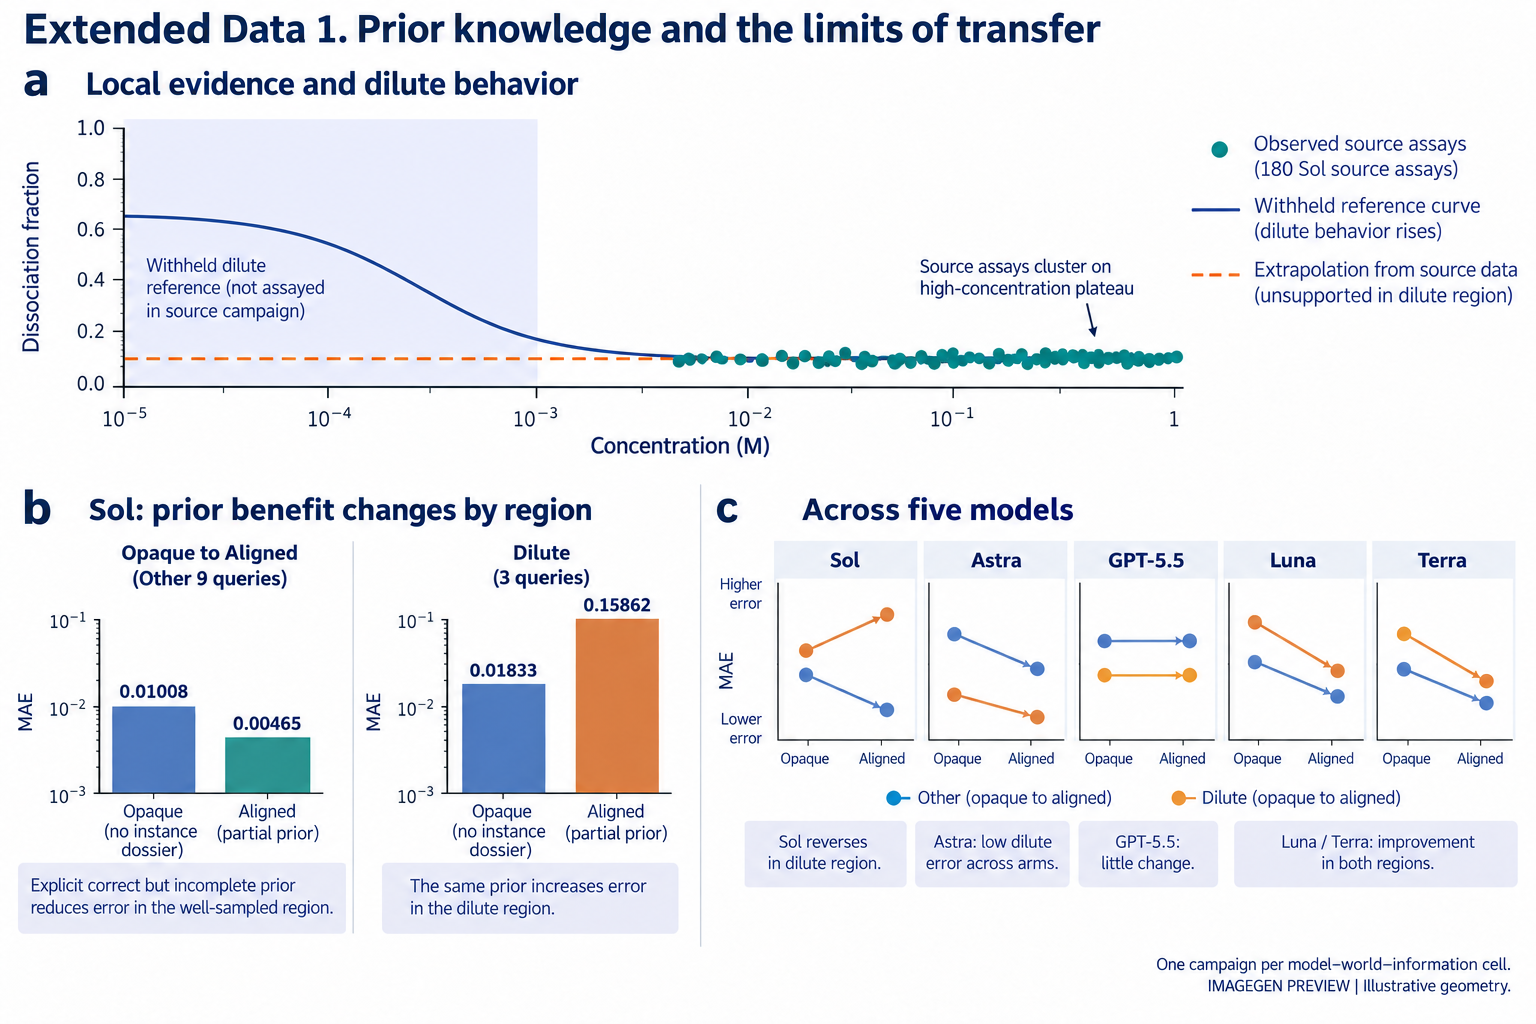
\includegraphics[width=\linewidth,height=.68\textheight,keepaspectratio]{../figures/imagegen-preview-20261016/ed01_priors.png}}
\caption{Extended Data Figure 1 \textbar{} Partial prior knowledge and transfer. a, Schematic local plateau, dilute reference behavior and an unsupported continuation. b, Historical Sol/Opaque versus Aligned errors in two query regions. c, Qualitative patterns across five models, not numerical effect estimates. Historical cells contain one campaign each; the dilute partition was post hoc in that cohort and fixed before subsequent repeated blocks. Repeated-cohort estimates are not pooled here. ImageGen preview: geometry is illustrative; exact values are in the retained evidence.}
\end{figure}

\clearpage\begin{figure}[H]
\centering
\pandocbounded{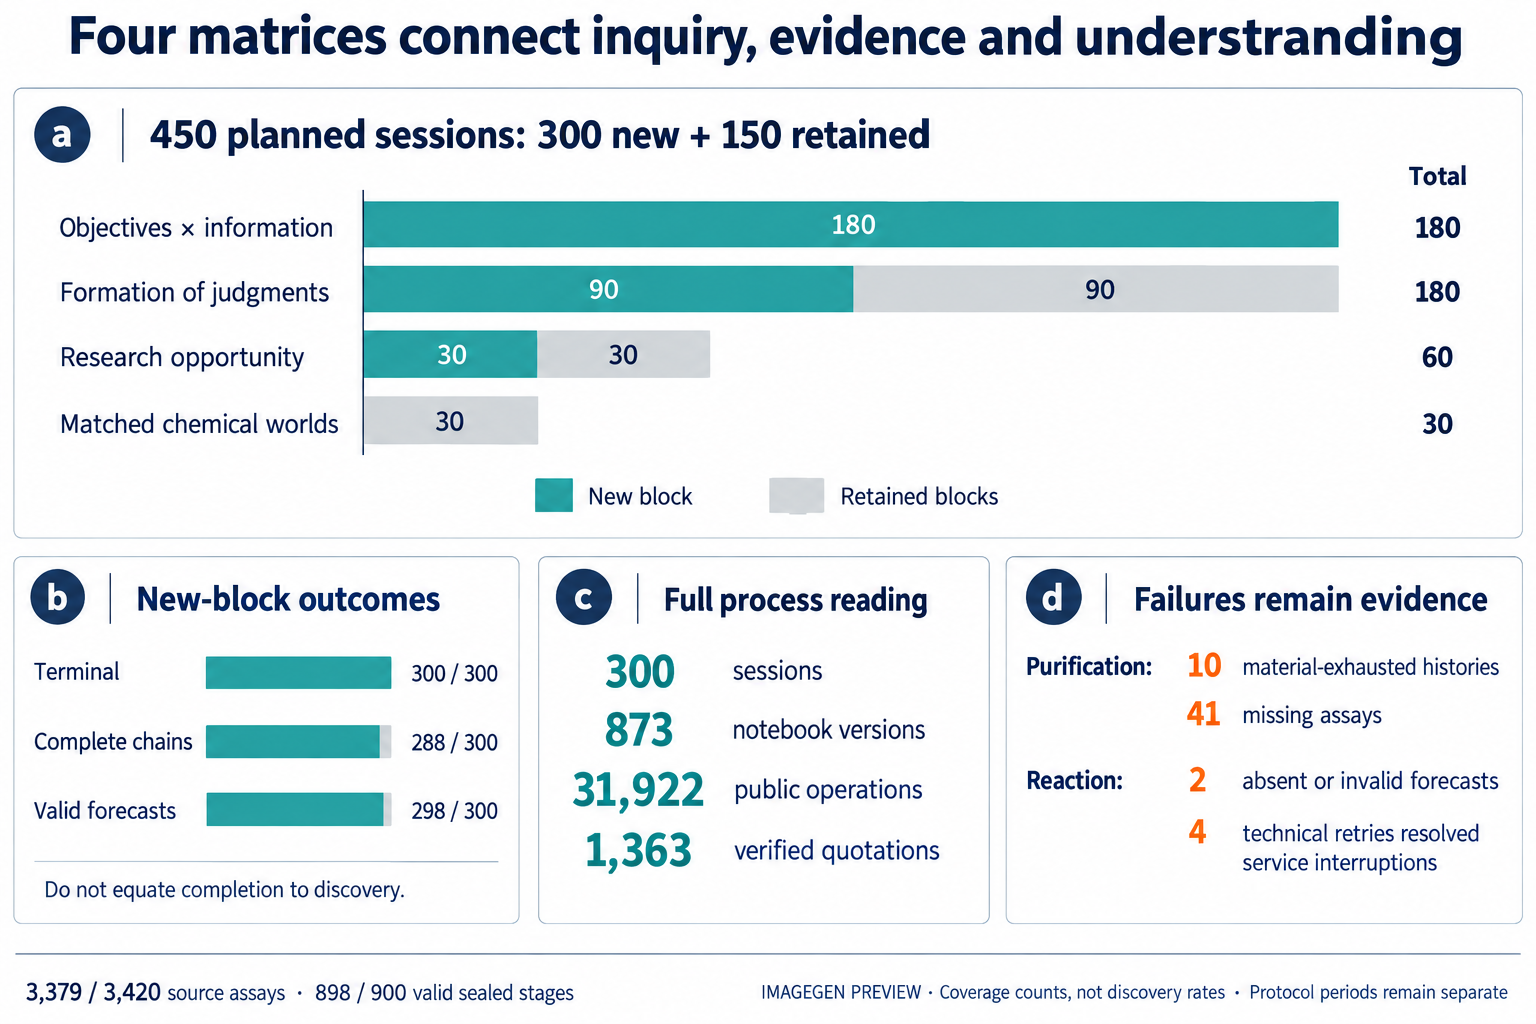
\includegraphics[width=\linewidth,height=.68\textheight,keepaspectratio]{../figures/imagegen-preview-20261017/ed02_coverage.png}}
\caption{Extended Data Figure 2 \textbar{} Integrated design and new-block coverage. a, Four matrices contain 450 planned sessions: 300 new and 150 retained under separate protocols. b, The new block retains 288 complete chains and 298 valid forecasts; completion is not scientific success. c, Full reading covers 873 notebook versions and 31,922 public operations, with 1,363 verified quotations. d, Ten purification histories miss forty-one assays after material exhaustion; two reaction forecasts are absent or invalid. Technical retries resolve four service interruptions without replacing scientific outcomes. ImageGen preview: geometry is illustrative.}
\end{figure}

\clearpage\begin{figure}[H]
\centering
\pandocbounded{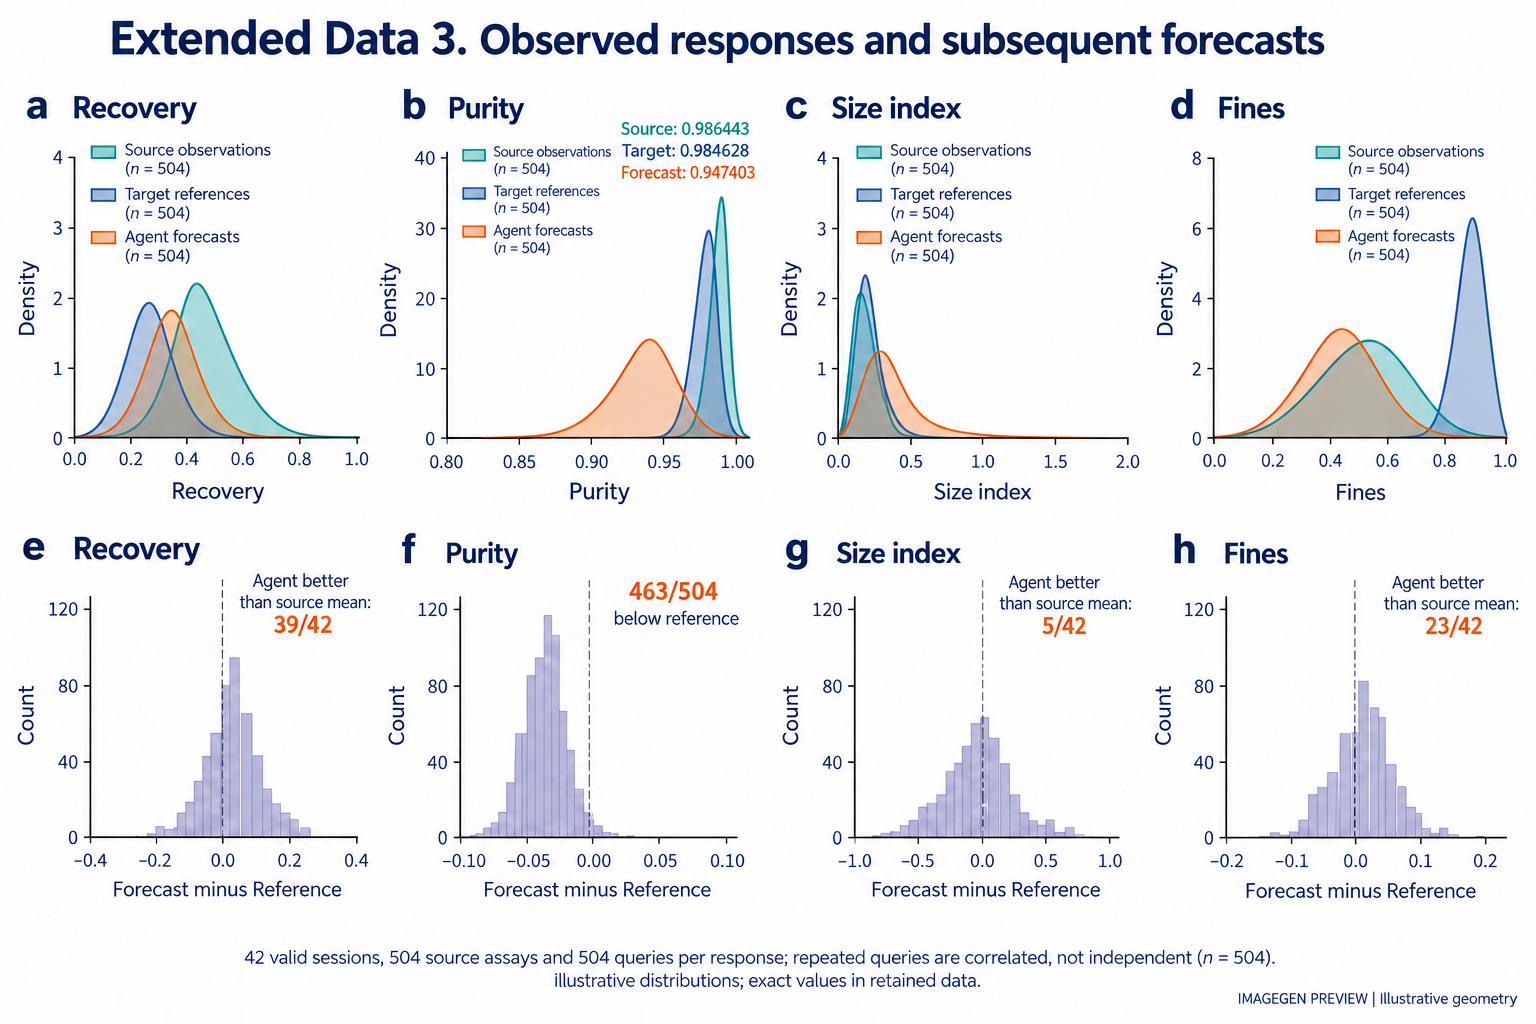
\includegraphics[width=\linewidth,height=.68\textheight,keepaspectratio]{../figures/imagegen-preview-20261016/ed03_distributions.png}}
\caption{Extended Data Figure 3 \textbar{} Corrected-crystallization response distributions. a--d, Illustrative distributions for source observations, reference targets and agent forecasts. e--h, Illustrative signed-error distributions; their geometry and bin counts are not observations. The retained cohort has 42 valid forecasts, 504 source assays and 504 queries per response; shared targets are not independent researcher samples. Numeric callouts retain source summaries. Size is a dimensionless index. Three missing forecasts remain in the planned denominator of 45. ImageGen preview: geometry is illustrative; exact values are in the retained evidence.}
\end{figure}

\clearpage\begin{figure}[H]
\centering
\pandocbounded{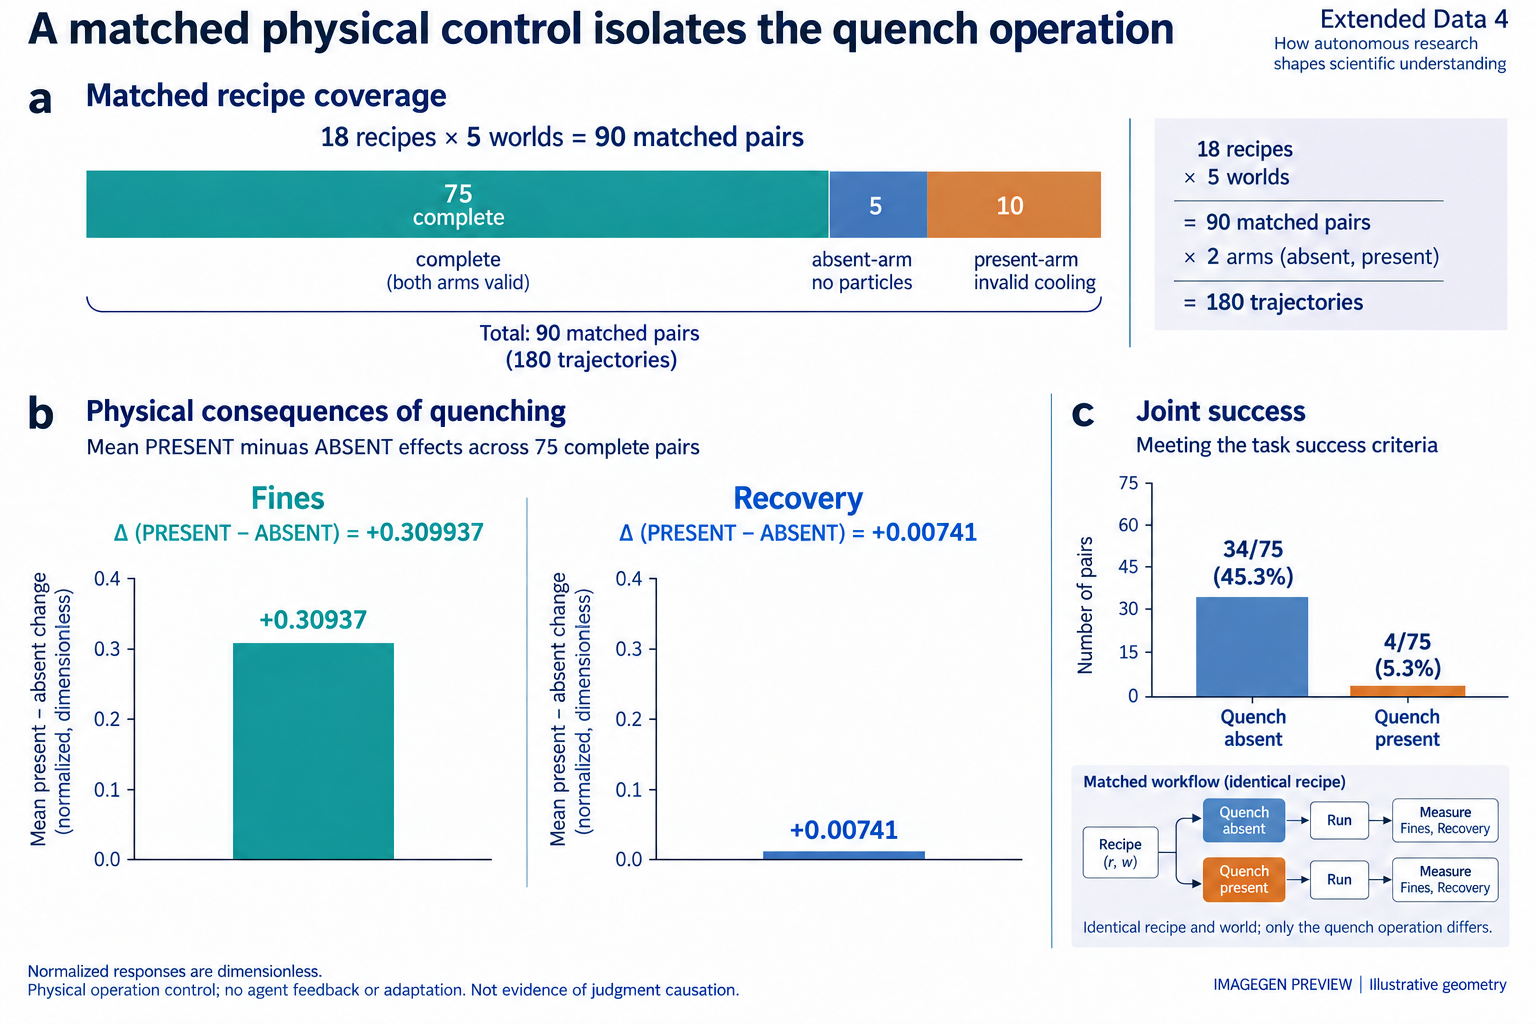
\includegraphics[width=\linewidth,height=.68\textheight,keepaspectratio]{../figures/imagegen-preview-20261016/ed04_quench.png}}
\caption{Extended Data Figure 4 \textbar{} Matched physical effects of quenching. a, Eighteen historical recipes across five worlds yield ninety pairs, with seventy-five complete, five absent arms lacking particles and ten present arms invalidating cooling. b, Mean present-minus-absent changes among complete pairs. c, Joint task success in those 75 pairs. These are physical effects under the implemented initial-charge recovery metric. Agents neither adapt nor receive these results, so no effect on judgment formation is inferred. ImageGen preview: geometry is illustrative; exact values are in the retained evidence.}
\end{figure}

\clearpage\begin{figure}[H]
\centering
\pandocbounded{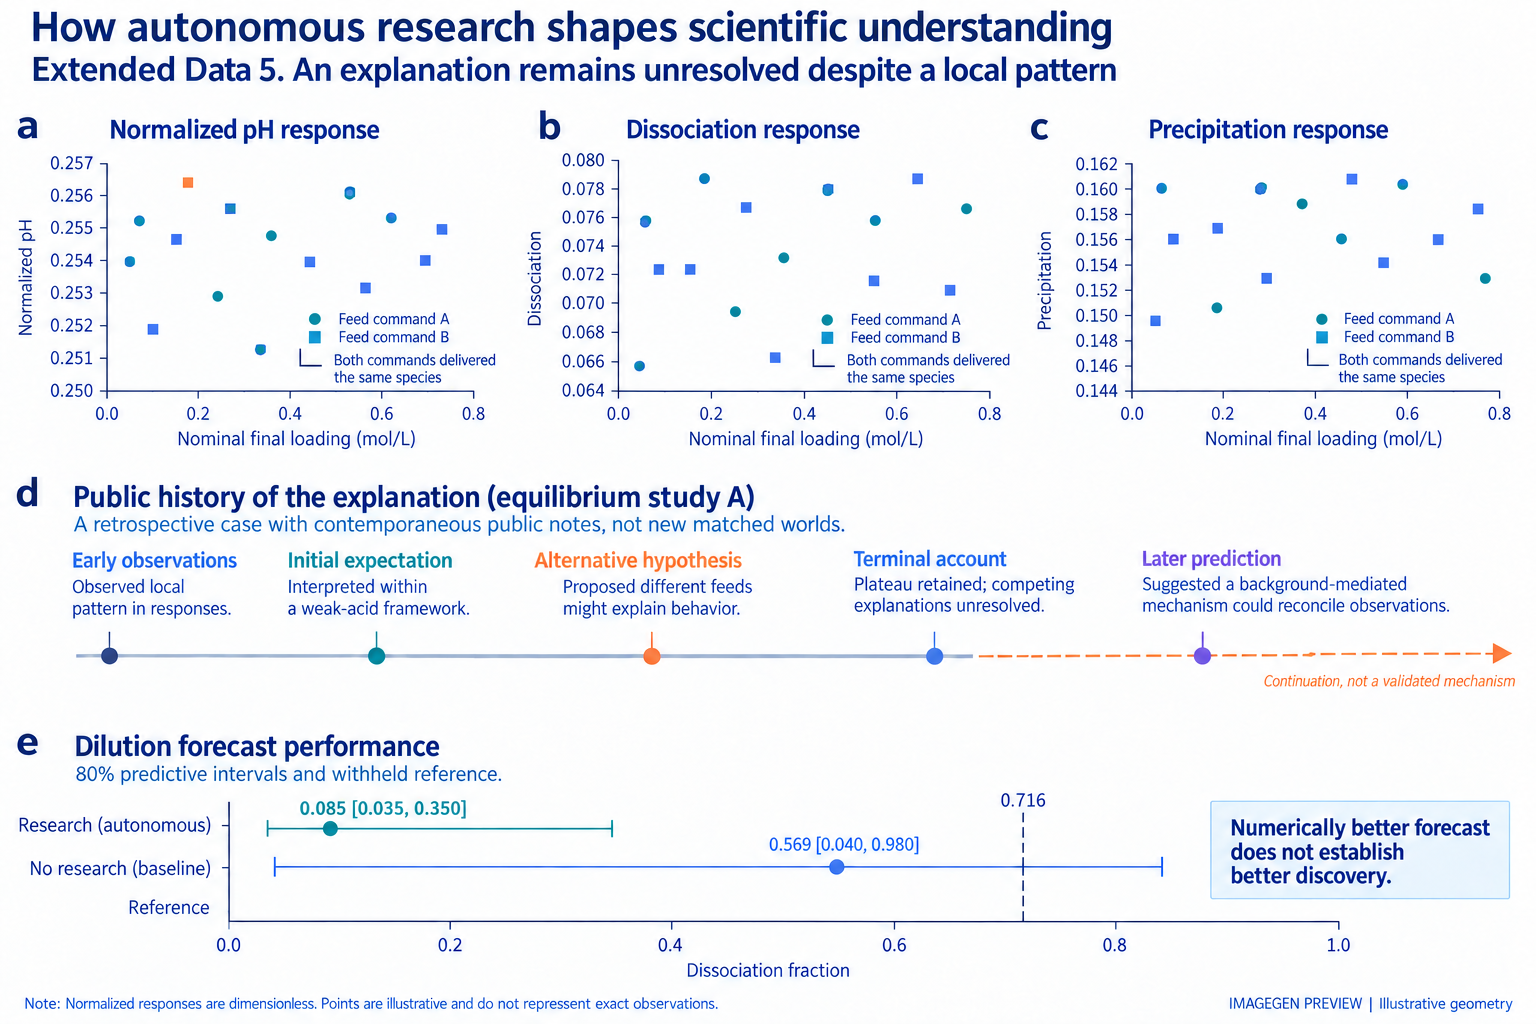
\includegraphics[width=\linewidth,height=.68\textheight,keepaspectratio]{../figures/imagegen-preview-20261016/ed05_history.png}}
\caption{Extended Data Figure 5 \textbar{} A local pattern and an unresolved explanation. a--c, Illustrative source-response patterns in equilibrium study A. Reagent and component commands add the same species in this execution version. d, The public history is condensed from an initial expectation through terminal uncertainty and later use; text is analytical summary, not quotations. e, Retained dilute dissociation forecasts, original 80\% predictive intervals and withheld mean. Numerical accuracy does not establish a discovery mechanism. ImageGen preview: geometry is illustrative; exact values are in the retained evidence.}
\end{figure}

\clearpage\begin{figure}[H]
\centering
\pandocbounded{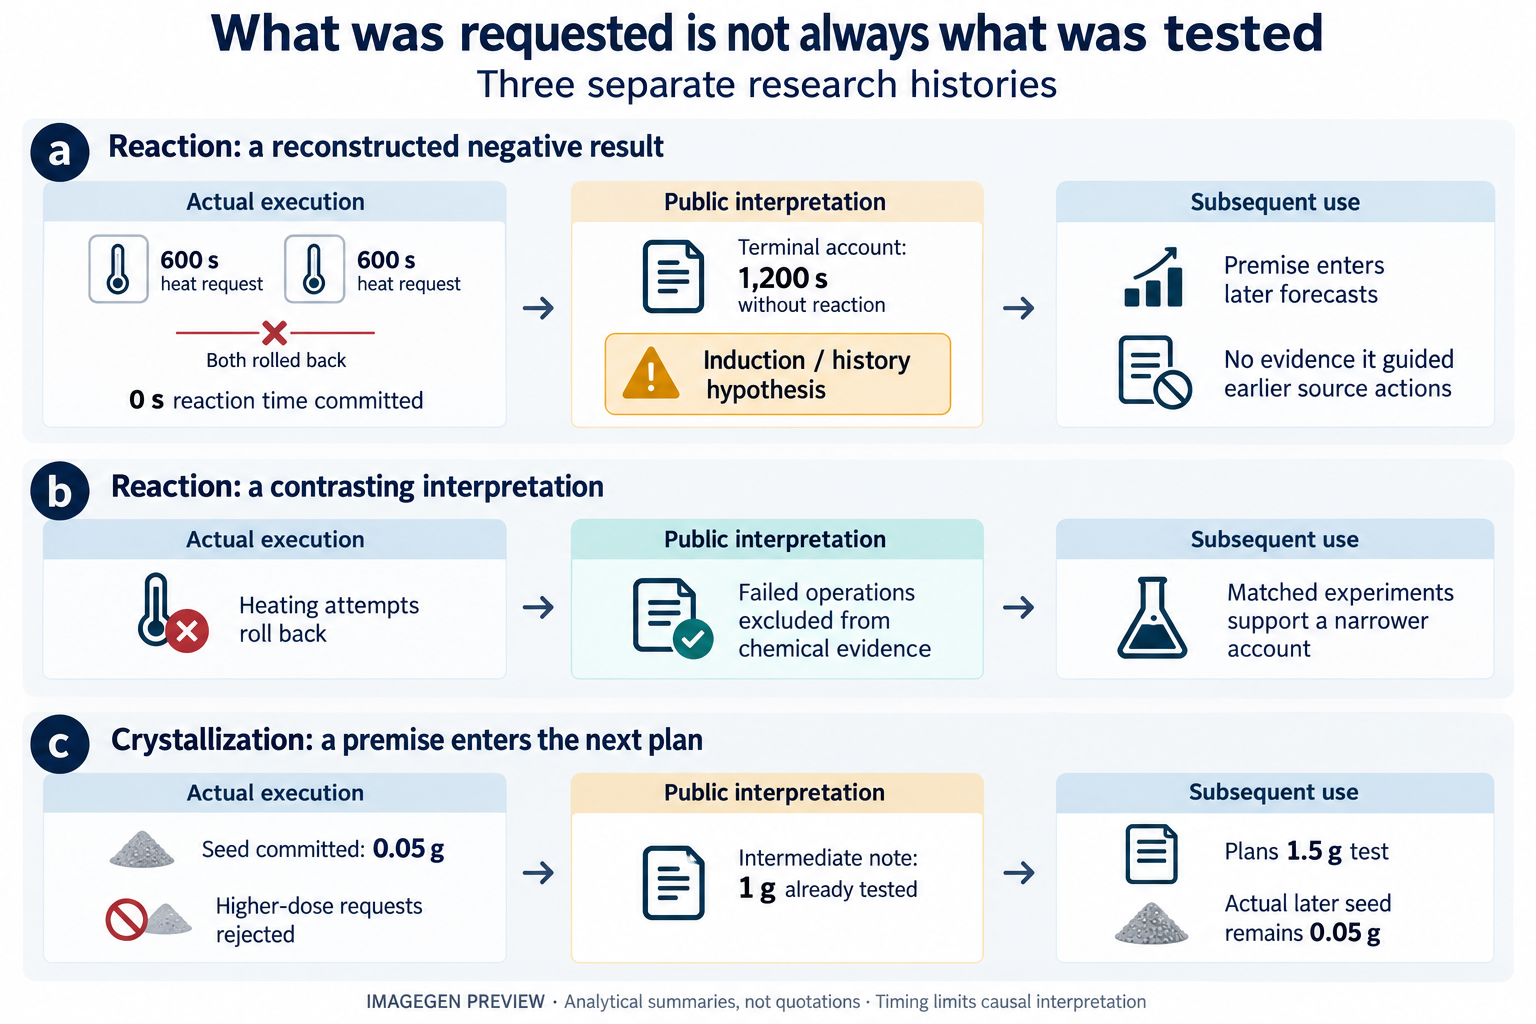
\includegraphics[width=\linewidth,height=.68\textheight,keepaspectratio]{../figures/imagegen-preview-20261017/ed06_reconstruction.png}}
\caption{Extended Data Figure 6 \textbar{} Reconstructing what the experiment tested. a, Two rolled-back heating requests become a claimed 1,200 s negative result in one terminal reaction account; subsequent predictions invoke an induction or history effect. b, Another session excludes rolled-back heating from chemical interpretation. c, An intermediate crystallization note reports a 1 g seed test despite 0.05 g committed, then proposes a higher dose. Timing distinguishes later forecast use from an observed influence on subsequent source actions. The focal heating return combines outer success/completion labels with an explicit rollback error and zero time/temperature changes. This is joint evidence about interface presentation and reconstruction of experience. Separate histories are not randomized correction arms. ImageGen preview: text is analytical summary, geometry illustrative.}
\end{figure}

\clearpage\begin{figure}[H]
\centering
\pandocbounded{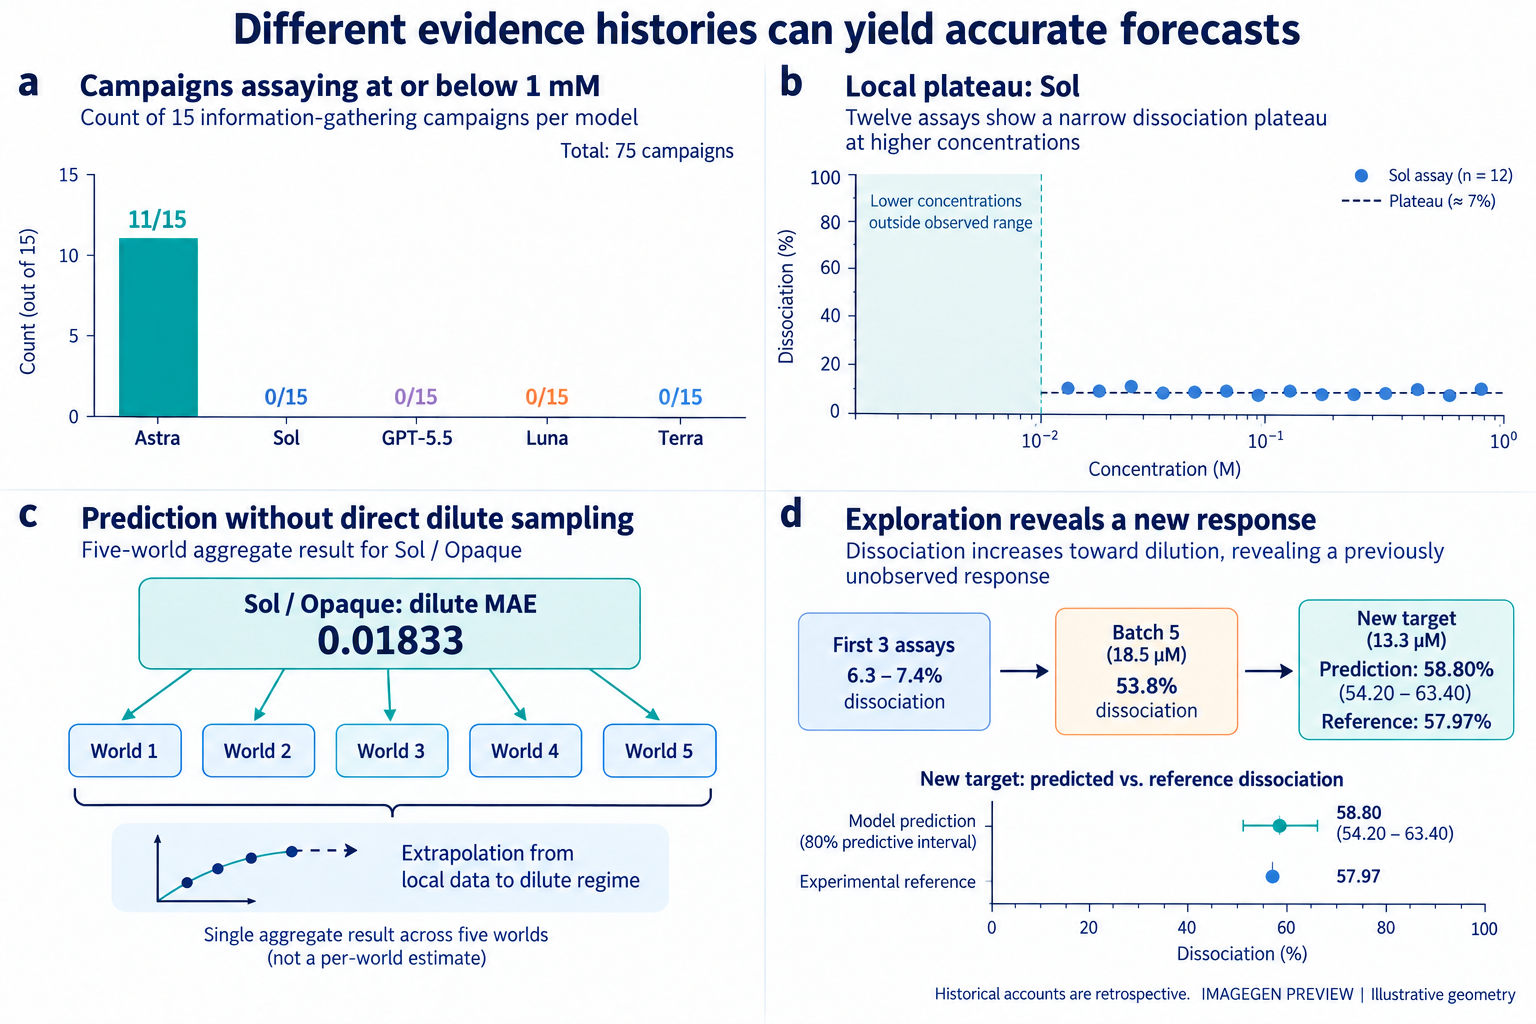
\includegraphics[width=\linewidth,height=.68\textheight,keepaspectratio]{../figures/imagegen-preview-20261016/fig03_paths.png}}
\caption{Extended Data Figure 7 \textbar{} Different routes from evidence to prediction. a, Campaigns reaching at or below 1 mM among fifteen per model. b, An illustrative local dissociation plateau. c, The five-world Sol/Opaque dilute MAE is an aggregate, not a separate value for each world. d, Selected stages of one Astra campaign and its sealed forecast, with the original 80\% predictive interval. Historical scientific accounts are retrospective. These observations do not establish fixed model traits. ImageGen preview: geometry is illustrative; exact values are in the retained evidence.}
\end{figure}

\clearpage\begin{figure}[H]
\centering
\pandocbounded{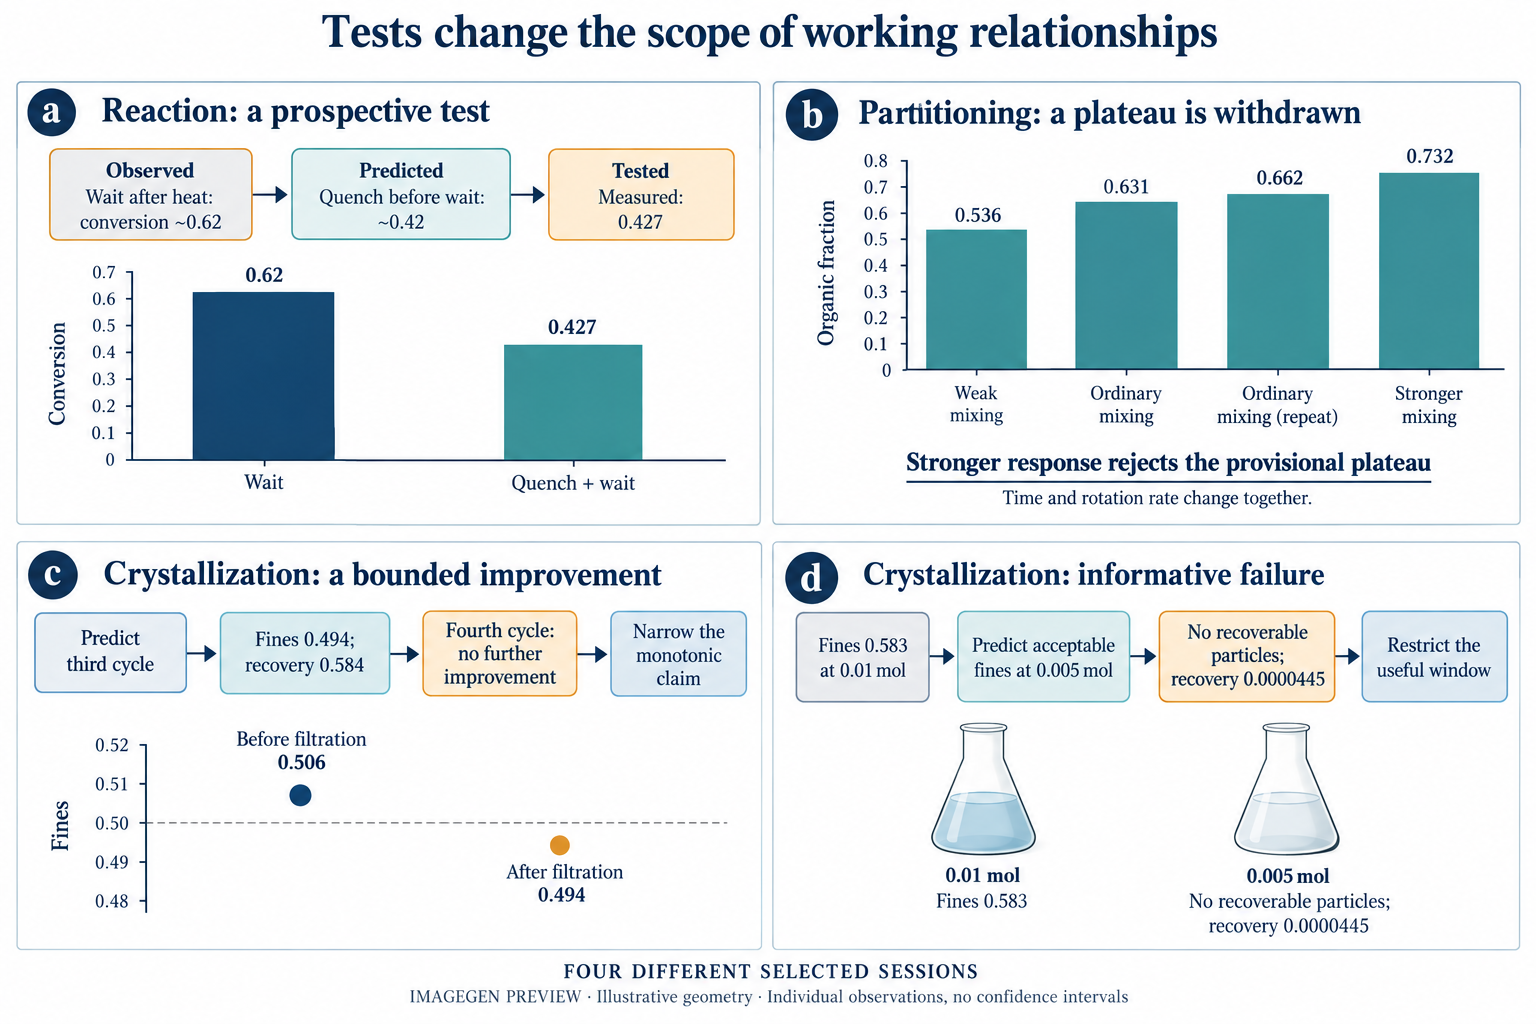
\includegraphics[width=\linewidth,height=.68\textheight,keepaspectratio]{../figures/imagegen-preview-20261017/fig05_revision.png}}
\caption{Extended Data Figure 8 \textbar{} Tests change the scope of working relationships. a, A prospective quench-before-wait prediction is followed by conversion 0.427, near the predicted 0.42. b, A stronger mixing condition leads to withdrawal of a provisional partitioning plateau; duration and rotation rate are confounded. c, A third crystallization cycle gives a near-threshold result, while a fourth fails to continue the improvement. d, Further dilution fails to preserve recoverable particles and narrows the proposed operating window. The panels are separate selected histories. Values are individual observations, not estimated treatment means or confidence intervals. ImageGen preview: geometry is illustrative; exact records accompany the manuscript.}
\end{figure}

\end{document}
